    \documentclass[a4paper,12pt,twoside]{ThesisStyle}
\usepackage[utf8]{inputenc}
\usepackage{thesis-style}
\usepackage[english]{babel}
\usepackage[T1]{fontenc}

\usepackage{subcaption}
\usepackage{graphicx}
\usepackage{enumitem} % Required for customizing itemize labels
\usepackage{enumitem}
\usepackage{fancyvrb}
\usepackage[toc,page]{appendix}
\usepackage{adjustbox}
\usepackage{pdflscape}
\usepackage{booktabs}% http://ctan.org/pkg/booktabs



\usepackage[table]{xcolor}
\definecolor{signaturegray}{gray}{0.98}

\RequirePackage{tikz}
\definecolor{ao}{rgb}{0.0, 0.5, 0.0}
\definecolor{darkpastelgreen}{rgb}{0.01, 0.75, 0.24}
\definecolor{amber}{rgb}{1.0, 0.75, 0.0}
\usetikzlibrary{mindmap}  % Mindmap drawing library

\setlength{\parindent}{0pt} % Drops all identation of all paragraphs

\begin{document}

\frontmatter

\pagenumbering{gobble}

\thispagestyle{empty}
\begin{table}[htb]
\centering
\begin{Large}
\resizebox{\textwidth}{!}{\begin{tabular}{ | l |}
 \hline
 \\
\includegraphics[scale=0.9]{imatges/logo_eps.png} \\[0.7cm]
\centerline{Treball Final de Màster}\\[1cm]
\hline
\\
Estudi: Màster en Ciència de Dades\\[0.7cm]
\hline
\\
Títol: Plataforma per Classificar Melanomes \\[0.7cm]
\hline
\\
Document: Memòria\\[0.7cm]
\hline
\\
Alumne: Wilber Eduardo Bermeo Quito \\[0.7cm]
\hline
\\
Tutor: Rafael Garcia Campos \\
Departament:  ARQUITECTURA I TECNOLOGIA DE COMPUTADORS \\
Àrea: ARQUITECTURA I TECNOLOGIA DE COMPUTADORS \\[0.7cm]
\hline
\\
Convocatòria (mes/any): Setembre 2022\\[0.7cm]
\hline

\end{tabular}}
\end{Large}
\end{table}

\newpage
\hypersetup{pageanchor=false}
\begin{titlepage}

% Upper part of the page
\includegraphics[scale=0.9]{imatges/logo_eps.png} \\[1cm]
\begin{center}
\textsc{\Large Master's thesis} \\[1cm]

% Title
\begin{spacing}{2}
\HRule \\
\textbf{\Huge A Platform for Classifying Melanoma} \\
\HRule \\[0.5cm]
\end{spacing}

% Author and supervisor and other data
{
\large
\textsc{Wilber Eduardo Bermeo Quito} \\
\small{September 2022} \\[0.75cm]
Master in Data Science \\[0.75cm]
\emph{Advisors:} \\[0.1cm]
\large
\textsc{Dr. Rafael Garcia Campos} \\
\small{Universitat de Girona} \\
\small{Departament of Computer Architecture and Technology} \\[0.5cm]

\large
\textsc{Sr. Luis Pla Llopis} \\
\small{Accenture S.L.} \\

}

\end{center}
\end{titlepage}
\hypersetup{pageanchor=true}

\titlepage

%\dominitoc


\pagenumbering{roman}

\chapter*{Summary}
%\label{cap:resum}

Skin cancer, including melanoma, is a significant global public health concern.
Melanoma presents a considerable challenge due to its high mortality rate and
the critical importance of early detection for successful treatment. Cancer
begins when healthy cells undergo changes that cause them to grow and divide
uncontrollably, forming tumors. These tumors can be classified as either
cancerous (malignant) or non-cancerous (benign). Malignant tumors have the
potential to invade nearby tissues and spread to other parts of the body
through metastasis. \\

In recent times, there has been a growing focus on automating tasks in the
medical field through Computer-Aided Diagnosis (CAD). However, integrating CAD
into the medical system remains a significant challenge. \\

The objective of this project is to explore the current state of deep learning
techniques in image detection and assess their applicability and reliability in
creating a real-time system capable of classifying melanoma images. \\

The investigation led to the training of eight different models based on
convolutional layers with pre-trained weights from ResNet18 in the ImageNet
dataset. These models were distinguished by applying various machine learning
techniques during the training process, including regularization, data
augmentation, and learning rate scheduling, along with hyper-parameter
configuration. \\

The resulting models were trained on an unbalanced dataset of eight different
classes, comprising twenty-five thousand real dermoscopy images. Validation was
performed using three thousand different samples during the training phase. To
evaluate the models, a holdout set scheme was used, where they were tested on
unseen data, using three thousand samples, achieving good results (Table
\ref{table:test-set-resume-metrics}). To validate and further test the models,
Test-Time augmentation was employed to emulate an ensemble of models on the
fly. \\

This project goes beyond pure investigation and includes engineering efforts to
make sophisticated knowledge accessible to a wider audience. A CAD
infrastructure, based on micro-services, was created to provide medical
professionals with a powerful tool for advanced diagnostic capabilities. This
infrastructure integrates the trained models with an API and a user interface
(UI), enabling professionals to improve patient care and outcomes. \\

The developed CAD infrastructure stands as a significant advancement in the
automation of melanoma detection, enhancing the potential for early diagnosis
and better patient outcomes. \\

The research's final conclusions can be summarized in two key points. Firstly,
there are significant benefits in developing platforms and infrastructure that
provide accessible machine learning solutions. Secondly, it is crucial to be
cautious when implementing certain machine learning solutions, as some "solved"
problems may raise moral and ethical concerns. \\

This project was carried out in partnership with the VICOROB
research group at the University of Girona and Accenture S.L. The documentation
and CAD infrastructure, along with the training and infrastructure code, are
freely accessible on GitHub at the following URL:
\url{https://github.com/wilberquito/melanoma.thesis}.


\chapter*{Gratitude}
%\label{cap:agraiments}

I would like to express my sincere gratitude to all those who have contributed to the completion of this thesis.
Their unwavering support, guidance, and encouragement have been invaluable throughout this academic journey. \\

First and foremost,
I extend my deepest appreciation to my thesis advisors, Dr. Rafael Garcia Campos and Sr. Luis Pla Llopis,
for their exceptional mentorship and insightful feedback.
Their expertise and dedication have been instrumental in shaping this research project and improving its quality. \\

Finally, I am profoundly grateful to my friends who eagerly took the time to read and review this thesis,
offering their valuable feedback to enhance its quality and depth.
Their willingness to invest their precious time and intellectual energy into providing constructive critiques
has been a tremendous source of support and motivation throughout this research journey.



\tableofcontents

\listoffigures

\listoftables

\mainmatter

% \chapter{Introduction}
\label{cap:intro}

\section{Problem Statement}

Skin cancer, including melanoma, represents a significant public health concern
worldwide. Melanoma, in particular, poses a considerable challenge due to its
high mortality rate and the need for early detection for successful treatment.
Early and correct diagnosis is key for ensuring patients have the best possible
prognosis. Misdiagnosis of melanoma leads to more pathology and dermatology
malpractice claims than any cancer except breast cancer, as an early
misdiagnosis can greatly reduce a patient's survival chances \cite{Melanoma}. \\

Dermoscopy, also known as dermatoscopy (Figure \ref{fig:procedure_dermoscopy}),
is a noninvasive technique widely utilized for the examination of cutaneous
lesions. It involves the use of a handheld instrument called a dermatoscope to
visualize subsurface skin structures that are typically not visible to the
naked eye. The dermatoscope illuminates the skin surface and provides
magnification, allowing for a detailed examination of the epidermis, the
dermoepidermal junction, and the papillary dermis. By analyzing these
structures, dermatologists can identify specific features and patterns
associated with various skin conditions, including melanoma \cite{Dermoscopy}.

\begin{figure}[htb] \centering
  \includegraphics[width=6cm]{imatges/introduction/medical_procedure_dermastocopy.jpeg}
  \caption[Dermoscopy Procedure]{\textit{Dermoscopy Procedure. Illustration by MD Anderson Cancer Center}}
  {\label{fig:procedure_dermoscopy}}
\end{figure}

Worldwide, in 2020 an estimated 324,635 people were diagnosed with melanoma and
an estimated 57,043 people worldwide died from melanoma the same year
\cite{CancerStats}. The introduction of sophisticated machinery and new
techniques in dermoscopy procedures (Figure \ref{fig:subset_isic}) seems not
enough to fight against melanoma, but the developments in artificial
intelligence (AI) especially in deep learning techniques, have made
Computer-Aided Diagnosis (CAD) a promising path towards
medical automation.

\begin{figure}[H] \centering
  \begin{subfigure}{0.3\textwidth}
    \includegraphics[width=\textwidth]{imatges/introduction/subset_isic/ISIC_1752943.jpg}
  \end{subfigure}
  \hfill
  \begin{subfigure}{0.3\textwidth}
    \includegraphics[width=\textwidth]{imatges/introduction/subset_isic/ISIC_1766619.jpg}
  \end{subfigure}
  \hfill
  \begin{subfigure}{0.3\textwidth}
    \includegraphics[width=\textwidth]{imatges/introduction/subset_isic/ISIC_1448526.jpg}
  \end{subfigure}
  \caption[Dermoscopy Images]{\textit{Dermoscopy Images. Illustration by ISIC Archive}}
  \label{fig:subset_isic}
\end{figure}

However, there are several limitations that raise doubts about the
effectiveness of automated melanoma cancer classifiers and their suitability
for integration into the medical system. Firstly, certain methods are
constructed based on theoretical models of melanoma appearance, which may
restrict their applicability to specific morphologies and fail to capture the
wide range of variations seen in real-world scenarios. Secondly, AI systems
utilized in these classifiers are trained to address a singular and narrow
task. Unlike human dermatologists, these systems lack the ability to consider
holistic patient information when formulating a final diagnosis, reflecting the
concept of weak AI \cite{WeakAI}. Lastly, numerous methods have been trained
and evaluated using high-quality image frames, which may result in instability
when applied under real-time conditions where image quality is often
compromised. A fundamental part of machine learning is the problem of
generalization, that is, how to make sure that a trained model performs well on
unseen data. If the unseen data has different distribution, i.e. a domain shift
exists, the problem is significantly more difficult; even the smallest changes
in the statistics as compared to the training data can cause a deep neural
network to fail completely \cite{DomainShift}. \\

Addressing these limitations and developing melanoma cancer classifiers that
encompass a wider range of morphologies, incorporate holistic patient
information, and demonstrate robustness in real-world scenarios are crucial for
improving the reliability and effectiveness of melanoma detection and diagnosis
systems.

\section{Project Objectives}

The main objective of this project is to create a health care infrastructure,
focused on melanoma detection using deep learning methods to train a system
capable of detecting melanoma on dermoscopy images to test the ability of
computer-assisted image analysis. To this end, the gradual achievements that
must be accomplished are:

\begin{itemize}
  \item Gaining a comprehensive understanding of the theory
    behind deep learning and its practical applications.
  \item Analyzing images
    from dermoscopy and acknowledge its most important features.
  \item Train
    deep learning models with different techniques based on tranfer-learning,
    exploiting images of the melanoma ISIC \footnote{International Skin Imaging
    Collaboration, an international effort to improve melanoma diagnosis.}
    Challenge \cite{IsicChallenge}.
  \item Developing a CAD infrastructure. The CAD infrastructure, should contain
    the already trained models with a simple web UI an API and finally a
    mechanism using Docker to create the images of the services making it ease
    to deploy in any based Linux System.
\end{itemize}

\section{Personal Motivation}

I envisioned this project as a unique fusion of three personal passions.
Firstly, I was fueled by a deep fascination with human cognition and reasoning.
Machines, in my eyes, represented a novel paradigm through which I could delve
further into this captivating realm. \\

I am also motivated by the remarkable problem-solving capacity of data.
Regardless of its structure, data holds immense potential to uncover hidden
patterns, provide insights, and drive innovation. The ability to extract
meaningful information from data, regardless of its form, inspires me to
constantly expand my knowledge and skills in order to contribute to the field
of data science and make a tangible difference in the world. \\

Last but not least, I am driven by the immense power of automation and its
ability to democratize access to research knowledge. I am amazed by how
automation processes can extract value and make them readily available to
professionals and the public alike.

\section{Statement of Originality}

I, Wilber Eduardo Bermeo Quito, declare that the thesis titled "A Platform for
Classifying Melanoma" is an original work completed with the support and
collaboration of Accenture SL and the VICOROB research group. \\

The content presented in this thesis is the outcome of my independent research
efforts, guided by the knowledge and expertise acquired through my academic
studies and the valuable contributions from Accenture S.L and the VICOROB
research group. \\

I acknowledge the importance of academic integrity and the consequences of
plagiarism. Hence, I affirm that all the information, data, results, figures,
and conclusions presented in this thesis are authentic and original. Any
references or sources used have been appropriately cited and referenced.

\section{Regulatory Framework}

The inclusion of legal considerations has become a significant aspect of the
field of medical imaging. Privacy concerns and the potential misuse of personal
information make sharing and distributing medical data particularly
challenging. To address these limitations, recent research collaborations have
focused on promoting the sharing of patient data through de-identification
methods. However, it is crucial to thoroughly analyze the obligations related
to the protection of individuals and their personal data before engaging in
projects involving medical imaging. \\

When working with medical images, it is the utmost importance to prioritize
patient privacy rights. In the context of developing a skin lesions database,
it is necessary to obtain signed consent from patients for the publication of
their data. For this thesis, the ISIC Archive database was utilized, this
database serves as a publicly accessible resource for teaching, research, and
the development and testing of diagnostic artificial intelligence algorithms,
and it resolves any concerns related to consent \cite{IsicArchive}. It is a
large and continually expanding open-source archive of skin images.

\section{Ethical Concern}

The outcome of this thesis is a melanoma classification tool, developed using
"black box" models. Although these well-trained models usually yield highly
accurate results, their lack of transparency poses a challenge in terms of
explainability. \\

The issue of explainability is a significant concern in this study since the
possibility of misclassification is considerable. When encountering a false
negative, it becomes crucial to understand the reasons behind the
misclassification. Consequently, both the introduction and conclusion of the
thesis emphasize that this tool is intended to assist human decision-making
rather than being an autonomous decision-making system.

\section{Contribution to Melanoma Detection}

In this section, we present our contribution to the field of melanoma
detection, which draws inspiration from related research in the development of
a melanoma CAD (Computer-Aided Diagnosis) infrastructure classifier. This
thesis is enriched by incorporating ideas from existing works and
state-of-the-art projects, which are elaborated in Chapter \ref{cap:estat}. \\

The thesis comprises multiple models employing various techniques, including
transfer learning, data augmentation, just-in-time testing, regularization, and
others. To compare these models, tools like W\&B (Weight \& Biases), a MLOps
platform for experiment tracking, and MLXTEND, providing utilities and
extensions for machine learning and data science in Python's scientific
computing stack, were utilized. The experiments were conducted using the ISIC
Archive dataset, consisting of benign and malignant skin lesions. Prior to
analysis, the dataset underwent preprocessing to enhance quality and normalize
features. Consequently, accurate classification and differentiation of melanoma
lesions from benign ones were achieved. \\

In order to to ensure the usability of the trained models,
two services were developed. These services include a user-friendly UI and an
API, both of which were containerized using Docker technology. By
containerizing the UI, an intuitive and interactive user experience was
provided, enabling users to seamlessly interact with the melanoma CAD system.
Similarly, containerizing the API streamlined request handling and prediction
serving, resulting in efficient performance. This approach facilitated easy
deployment across various platforms.

%
% \chapter{Related Work and State of the Art}
\label{cap:estat}

Melanoma, a type of cancer that arises from melanin-producing cells, can be
found in various parts of the body such as the skin, eyes, nerve centers, and
meninges. Early diagnosis is crucial for improving the chances of curing
melanoma, even though it has the highest increasing incidence rate among all
skin cancer types. According to a study \cite{TimelyMelanomaDetection}, timely
identification of early-stage skin cancer resulted in a significant 90\%
reduction in mortality rates. For instance, patients diagnosed with stage I
melanoma have a 10-year overall survival probability ranging from 94\% to 98\%,
while those in stage IV have a much lower estimated 10-year overall survival
rate of just 10\% to 15\%. \\

Dermoscopy is a non-surgical method used to examine the underlying layers of
the skin. While it can yield good results, it requires extensive training and
experience in dermatology. However, it may not provide a definitive diagnosis
for melanoma, especially in its early stages. Consequently, there is a need for
an automated diagnostic tool. \\

In \cite{EpidemiologySkinCancer} study, the melanoma task classification was
compared between expert opinions and artificial neural networks. The computer
program demonstrated had an area under the receiver operating characteristic
curve of 0.87, which was higher than the dermatologists (0.74), the program
also had a higher sensitivity in classification of 85\% against the 76\% by the
dermatologists. These findings indicate the potential utilization of automated
systems in the field of skin cancer detection. \\

For cancer prediction, a supervised learning approach is employed. The most
common algorithms or methodologies include decision trees, convolutional neural
networks (CNN), support vector machines (SVM), k-nearest neighbors (KNN) and
Transformers. One of the most powerful systems are CNNs (Convolutional Neural
Networks), despite the fact that their use may involve a loss of
explainability, which is a major concern in healthcare systems. \\

Although this project goes beyond the mere creation of highly accurate models
for classifying melanoma, we have taken into consideration and reviewed related
works that have influenced and guided our own path.

\section{Identifying Melanoma Images Using EfficientNet Ensemble}

The winning approach to the 2020 SIIM-ISIC Melanoma Classification Challenge
\cite{ISICKaggle}. The team not only let the competition source code available
on GitHub \cite{WinningISICGithub} but they also wrote a paper explaining in
detail their investigation \cite{WinningISIC}. \\

The SIIM-ISIC Melanoma Classification Challenge was conquered by this ensemble of
convolutional neural networks (CNN). The winning solution involved training 16
EfficientNets, along with a ResNext101 and a ResNet101. To create this ensemble
of models, various strategies were employed, including utilizing patients'
metadata in addition to dermoscopy images, training models with different input
image sizes, and even training the models for varying numbers of epochs
\cite{WinningISIC}.

\begin{itemize}
  \item Implementation of a stable validation scheme.
  \item Effective selection of the model target.
  \item Thoughtful optimization of the pipeline.
  \item Utilization of ensemble learning with highly diverse models.
\end{itemize}

The submission that won achieved an AUC (Area Under the Curve)\footnote{AUC is
a metric that quantifies the overall quality of a binary classification model
by measuring the area under its ROC curve. It provides a single value that
summarizes the model's ability to discriminate between positive and negative
instances.} score of 0.9600 on cross-validation and 0.9490 on the private
leaderboard. \\

From their work, we adopted various deep learning techniques. For instance, we
applied the same way they evaluate models given an unbalanced multi-class
data-sets like as the ISIC dataset is. To properly assess the training process,
they utilized the AUC with one-vs-rest (OvR) metric. This project as well uses
this metric to evaluate the performance of the models. \\

Another aspect the current thesis borrowed from this work is the approach to
cleaning and mapping data-sets from different years. They trained their models
with different input image sizes, but the process of mapping and joining the
data-sets into a single data-set was similar to our approach, where we
consistently mapped the data into eight different classes. \\

The pipeline of data augmentation that is implemented in the work is also
reused. Equivalent to them, this thesis uses {\tt
albumentations}\cite{Albumentations} library instead of the native data
agumentation package provided from PyTorch. \\

These inspirations and adaptations from the related work has greatly influenced
the development and organization of this deep learning project.

\section{CNN Explainer}

CNN explainer is a web page created through a collaborative research effort
between Georgia Tech and Oregon State\cite{CNNExplainer}. It leverages
TensorFlow.js, a deep learning library that utilizes GPU acceleration within
the web browser, to load pretrained models for visualization. The entire
interactive system is implemented in JavaScript, utilizing Svelte as a
framework and D3.js for visualizations. With CNN Explainer, users can upload
images and obtain predictions for those images across ten different classes.
\\

While CNN Explainer primarily aims to serve educational purposes, the UI of the
current thesis, focuses on providing dermoscopy images predictions and
information about the models used and their outputs. The inspiration for
incorporating an interactive UI for end users stemmed from CNN Explainer.
Consequently, we utilized the same web framework to develop the UI.

\section{Dermatologist-level Classification of Skin Cancer with
Deep Neural Networks}

This study demonstrated the use of a deep learning algorithm to classify skin
lesions, including melanoma, with accuracy comparable to dermatologists. The
deep neural network was trained on a large dataset of images and achieved high
sensitivity and specificity \cite{SkinCancerDeepNN}.

\section{Computerized Analysis of Pigmented Skin Lesions: A
Review}

The goal of this paper is to review the papers on computerized analysis of
dermoscopy and clinical images of pigmented skin lesions. The paper also
clarifies terminology that is often misused in the literature, and it also
organizes and group together useful sources, making it easier to find
information on a particular sub-topic when searching through the existing
literature \cite{MelanomaTopicsReview}.

%
% \chapter{Domain} \label{cap:problem_domain}

In this chapter, we will delve into the details of melanoma cancer, including
its origins, factors contributing to its development, and strategies to
minimize the risk of its occurrence. Additionally, we will explore other common
types of skin cancer and their underlying causes. \\

By the end of this chapter, our aim is to provide a comprehensive understanding
of this condition, equipping you with the knowledge necessary to comprehend the
proposed solution in this thesis.

\section{The Skin}

The skin, which is our body's largest organ \cite{BaseCancerKnowledge}, plays a
crucial role in safeguarding us against external threats and maintaining our
overall health. It consists of several layers (Figure
\ref{fig:melanoma_diagram}), with the main layers being:

\begin{itemize} \item \textbf{Epidermis}

      The epidermis is the outermost layer of the skin, serving as a protective
      shield against environmental factors. It consists mainly of flat,
      scale-like cells called keratinocytes. These cells produce a tough
      protein called keratin, which helps make the skin waterproof and
      resistant to damage. Within the epidermis, specialized cells called
      melanocytes produce melanin, the pigment responsible for skin color.
      Melanin also helps protect the skin from harmful ultraviolet (UV)
      radiation. \\

      The epidermis is made up of several layers, including the stratum
      corneum, the topmost layer composed of dead skin cells that are
      continuously shed and replaced by new cells from the lower layers. The
      epidermis also contains other types of cells, such as Langerhans cells,
      which are part of the immune system and help defend against infections.

      \newpage

    \item \textbf{Dermis}

      Beneath the epidermis lies the dermis, a complex layer that provides
      structural support to the skin. The dermis contains a network of blood
      vessels that supply nutrients and oxygen to the skin cells. It also
      houses various structures, including hair follicles, sweat glands,
      sebaceous glands, and nerve endings. The dermis is composed of collagen
      and elastin fibers, which give the skin its strength, elasticity, and
      flexibility. These fibers allow the skin to stretch and recoil as needed.
      The dermis also plays a crucial role in thermoregulation by regulating
      blood flow to control body temperature.

    \item \textbf{Hypodermis (Subcutaneous Tissue)}

      The deepest layer of the skin is called the hypodermis or subcutaneous
      tissue. It is primarily made up of adipose tissue, which provides
      insulation, cushioning, and energy storage. The hypodermis helps to
      regulate body temperature by acting as an insulating layer, preventing
      heat loss. It also acts as a shock absorber, protecting the underlying
      structures and organs from injury. Additionally, the hypodermis serves as
      a connection between the skin and the underlying muscles and bones. It
      contains blood vessels and nerve endings that supply nutrients and
      sensations to the skin.

\end{itemize}

\begin{figure}[H] \centering
  \includegraphics[width=0.85\textwidth]{imatges/problem_domain/melanoma-diagram.jpg}
  \caption[Skin Main Layers]{\textit{Skin Main Layers. Illustration by
Cancer.Net}} {\label{fig:melanoma_diagram}} \end{figure}

\section{Skin Cancer}

Cancer begins when healthy cells undergo changes that cause them to grow and
divide uncontrollably, forming a mass known as a tumor. Tumors can be
classified as either cancerous or benign. A cancerous tumor is considered
malignant, meaning it has the potential to invade nearby tissues and spread to
other parts of the body through a process called metastasis. Conversely, a
benign tumor may grow locally but does not have the ability to spread to other
areas. \\

Skin cancer is one of the most prevalent types of cancer, with over 3 million
Americans diagnosed each year. However, the prognosis for skin cancer is
generally favorable when detected early. Treatment options for skin cancer
often involve topical medications, in-office procedures performed by
dermatologists, or outpatient surgeries. Dermatologists specialize in
diagnosing and treating conditions of the skin. As a result, skin cancer
accounts for less than 1\% of all cancer-related deaths. \\

In more advanced cases, skin cancer may require comprehensive medical care
provided by a multidisciplinary team, which typically includes a dermatologist,
surgical oncologist, radiation oncologist, and clinical oncologist.

\subsection{Types of Skin Cancer}

There are three primary forms of skin cancer \cite{BaseCancerKnowledge}.

\begin{itemize}

  \item \textbf{Basal cell carcinoma}

    This type of skin cancer arises from basal cells located in the lower
    epidermis. Approximately 80\% to 90\% of skin cancers originate from
    these cells, leading to the designation of basal cell carcinomas. They
    typically develop on the head and neck, although they can occur anywhere
    on the skin. Sun exposure is the primary cause, although they may also
    occur in individuals who underwent radiation therapy during childhood.
    This type of skin cancer generally grows slowly and rarely metastasizes
    to other parts of the body.

  \item \textbf{Squamous cell carcinoma}

    This type of skin cancer originates from flat, scale-like cells known as
    squamous cells that comprise a significant portion of the epidermis.
    Around 10\% to 20\% of skin cancers develop from these cells, resulting
    in the classification of squamous cell carcinomas. Sun exposure is the
    main cause, and they can be diagnosed on various regions of the skin.
    They may also emerge on skin that has been burned, damaged by chemicals,
    or exposed to x-rays. Common sites for squamous cell carcinoma include
    the lips, areas with long-standing scars, and the skin surrounding the
    mouth, anus, and vagina. Roughly 2\% to 5\% of squamous cell carcinomas
    metastasize to other parts of the body.

  \item \textbf{Melanoma}

    The most aggressive type of skin cancer, originates in scattered cells
    known as melanocytes where the epidermis and dermis meet. Melanocytes
    produce the pigment melanin, responsible for skin color. Melanoma
    accounts for approximately 1\% of all skin cancers.

\end{itemize}

\subsection{Stages of Skin Cancer}

The following stages are used for basal cell carcinoma. Basal cell carcinoma
accounts for more than 90\% of all skin cancers in the United States and is the
most common of all cancers. Typically, it is a slow-growing cancer that seldom
spreads to other parts of the body \cite{CancerInstitute}. \\

\begin{itemize}

  \item \textbf{Stage I}

    In stage I, abnormal cells are found in the squamous cell or basal cell
    layer of the epidermis. These abnormal cells may become cancer and spread
    into nearby normal tissue.

    \begin{figure}[H] \centering
      \includegraphics[width=0.6\textwidth]{imatges/problem_domain/phase0-skin-cancer.jpg}
      \caption[Skin Cancer, Stage I]{\textit{Skin Cancer, Stage I. Illustration by Terese Winslow}}
    {\label{fig:stage0-skin-canceer}} \end{figure}

    \newpage


  \item \textbf{Stage II}

    In stage II, cancer has formed and the tumor is 2 centimeters or smaller.

    \begin{figure}[H] \centering
      \includegraphics[width=0.6\textwidth]{imatges/problem_domain/stage1-skin-cancer.jpg}
      \caption[Skin Cancer, Stage II]{\textit{Skin Cancer, Stage II.
      Illustration by Terese Winslow}} {\label{fig:stage1-skin-canceer}}
    \end{figure}


  \item \textbf{Stage III}

    In stage II, the tumor is larger than 2 centimeters but not larger than 4
    centimeters.

    \begin{figure}[H] \centering
      \includegraphics[width=0.6\textwidth]{imatges/problem_domain/stage2-skin-cancer.jpg}
      \caption[Skin Cancer, Stage III]{\textit{Skin Cancer, Stage III.
      Illustration by Terese Winslow}} {\label{fig:stage2-skin-canceer}}
    \end{figure}

    \newpage

  \item \textbf{Stage IV}

    In this stage, the cancer may spread to the rest of the body covering the
    nerves bellow the dermis or bellow the subcutaneous tissue or the bones.

    \begin{figure}[H] \centering
      \includegraphics[width=0.6\textwidth]{imatges/problem_domain/stage3-skin-cancer.jpg}
      \caption[Skin Cancer, Stage IV]{\textit{Skin Cancer, Stage IV. Illustration by
    Terese Winslow}} {\label{fig:stage3-skin-canceer}} \end{figure}

\end{itemize}

\subsection{Associated Factors and Prevention of Skin Cancer}

The risk factors associated with skin cancer encompass sun exposure, fair skin,
as well as certain physical characteristics such as blond hair and blue eyes.
The presence of melanin, a protein responsible for the skin's color or pigment,
plays a crucial role in shielding the skin from ultraviolet (UV) radiation.
Consequently, individuals with lighter skin or lower levels of melanin possess
reduced UV protection \cite{OrigenAndTreatment}. \\

Although skin cancer may initially appear to predominantly affect individuals
with light complexions, those with dark skin are also susceptible. They may
observe signs of cancer on the palms of their hands or soles of their feet.
\\

Advancements in research have led to treatments targeting the genetic level.
New drug therapies assist in stimulating the immune system to produce
antibodies capable of combatting rapidly dividing cells. While these therapies
may have potential side effects, they are generally milder than those
associated with chemotherapy. Moreover, they result in an enhanced immune
system that is better equipped to battle cancer. \\

A patient's overall health also appears to influence their ability to fight
cancer, although the precise connection between one's health and their risk of
developing cancer remains unclear. However, it can be assumed that better
overall health enhances the immune system's capacity to combat cancer. \\

Prevention of skin cancer is straightforward: minimizing exposure to the sun
and UV radiation. Ceasing the use of tanning beds is advised. When exposed to
the sun, wearing sunscreen and a wide-brimmed hat that provides comprehensive
head shading is recommended \cite{OrigenAndTreatment}. \\

Consideration should also be given to wearing clothing with SPF protection.
Some clothing manufacturers now produce summer attire with SPF levels similar
to those found in sunscreen. This is significant since most regular t-shirts
offer only minimal SPF protection of around 2. \\

Skin cancer ranks among the most prevalent forms of cancer, yet it is also one
of the most easily detectable and treatable. Taking proactive measures to
prevent sun exposure is crucial, while early detection is highly important. The
prognosis is favorable when melanoma is identified in its early stages.


\chapter{Preliminaries}
\label{cap:prelim}

The objective of this chapter is to provide a comprehensive overview that
defines the scope of the thesis. It covers essential theoretical and technical
concepts necessary to comprehend the experiments and the architecture proposed
in subsequent chapters.

\section{Artificial Intelligence}

\textit{AI} is one of the newest fields in science and engineering. Work
started in earnest soon after World War II, and the name itself was coined in
1956 attributed by John McCarthy of MIT. \\

After successfully decrypting Enigma\footnote{Enigma was a rotor machine
designed to encrypt and decrypt messages.}, in World War II, the mathematician
Alan Turing posed a groundbreaking question that had a profound impact on
society: "Can machines think?" \cite{CanMachineThink}. In this seminal work,
Turing not only outlined the process of developing intelligent machines but
also presented a method for assessing their intelligence. Even today, the
Turing Test remains a widely recognized benchmark for evaluating the
intelligence of artificial systems. According to this test, if a human cannot
distinguish, through a text-based conversation, whether they are interacting
with a human or a machine, the artificial system can be considered to possess
intelligence. \\

The term "AI" is exciting but, the definition of this term is blurry
\cite{AIModernApprouch}. Historically there are two approaches to \textit{AI}
that have been followed, each by different people with different methods. The
human-centered approach and the rationalist approach. The incorporation of a
human-centered approach into the field must incorporate empirical scientific
methods, which entail making observations and formulating hypotheses about
human behavior. On the other hand, a rationalist approach combines the
disciplines of mathematics and engineering. These different perspectives have
both faced criticism and received praises. \\

From that juncture until the turn of the century, the field of \textit{AI}
encountered fluctuations, witnessing periods of remarkable accomplishments
interspersed with the infamous \textit{AI} winters. Currently \textit{AI} is a
hot topic of discussion, evident from the increasing searches and online
mentions. While \textit{AI} has been around for more than 65 years, the recent
exponential trend can be attributed to the availability of cost-efficient
storage, transfer, and computation capabilities for massive amounts of data.
This newfound capacity was previously unimaginable and has contributed to the
current \textit{AI} boom. \\

\textit{AI} has expanded into numerous distinct fields, showcasing its
extensive range of applications, techniques, and interdisciplinary nature. The
diversity of branches in the field of artificial intelligence is represented in
Figure \ref{fig:ai_branches}, which depicts several current
\textit{AI} fields. However, it is important to note that the figure can be
further expanded to include additional fields, such as Speech Processing and
Expert Systems, among others.

\begin{figure}[H]
  \centering
  \resizebox{0.8\textwidth}{!}{%
    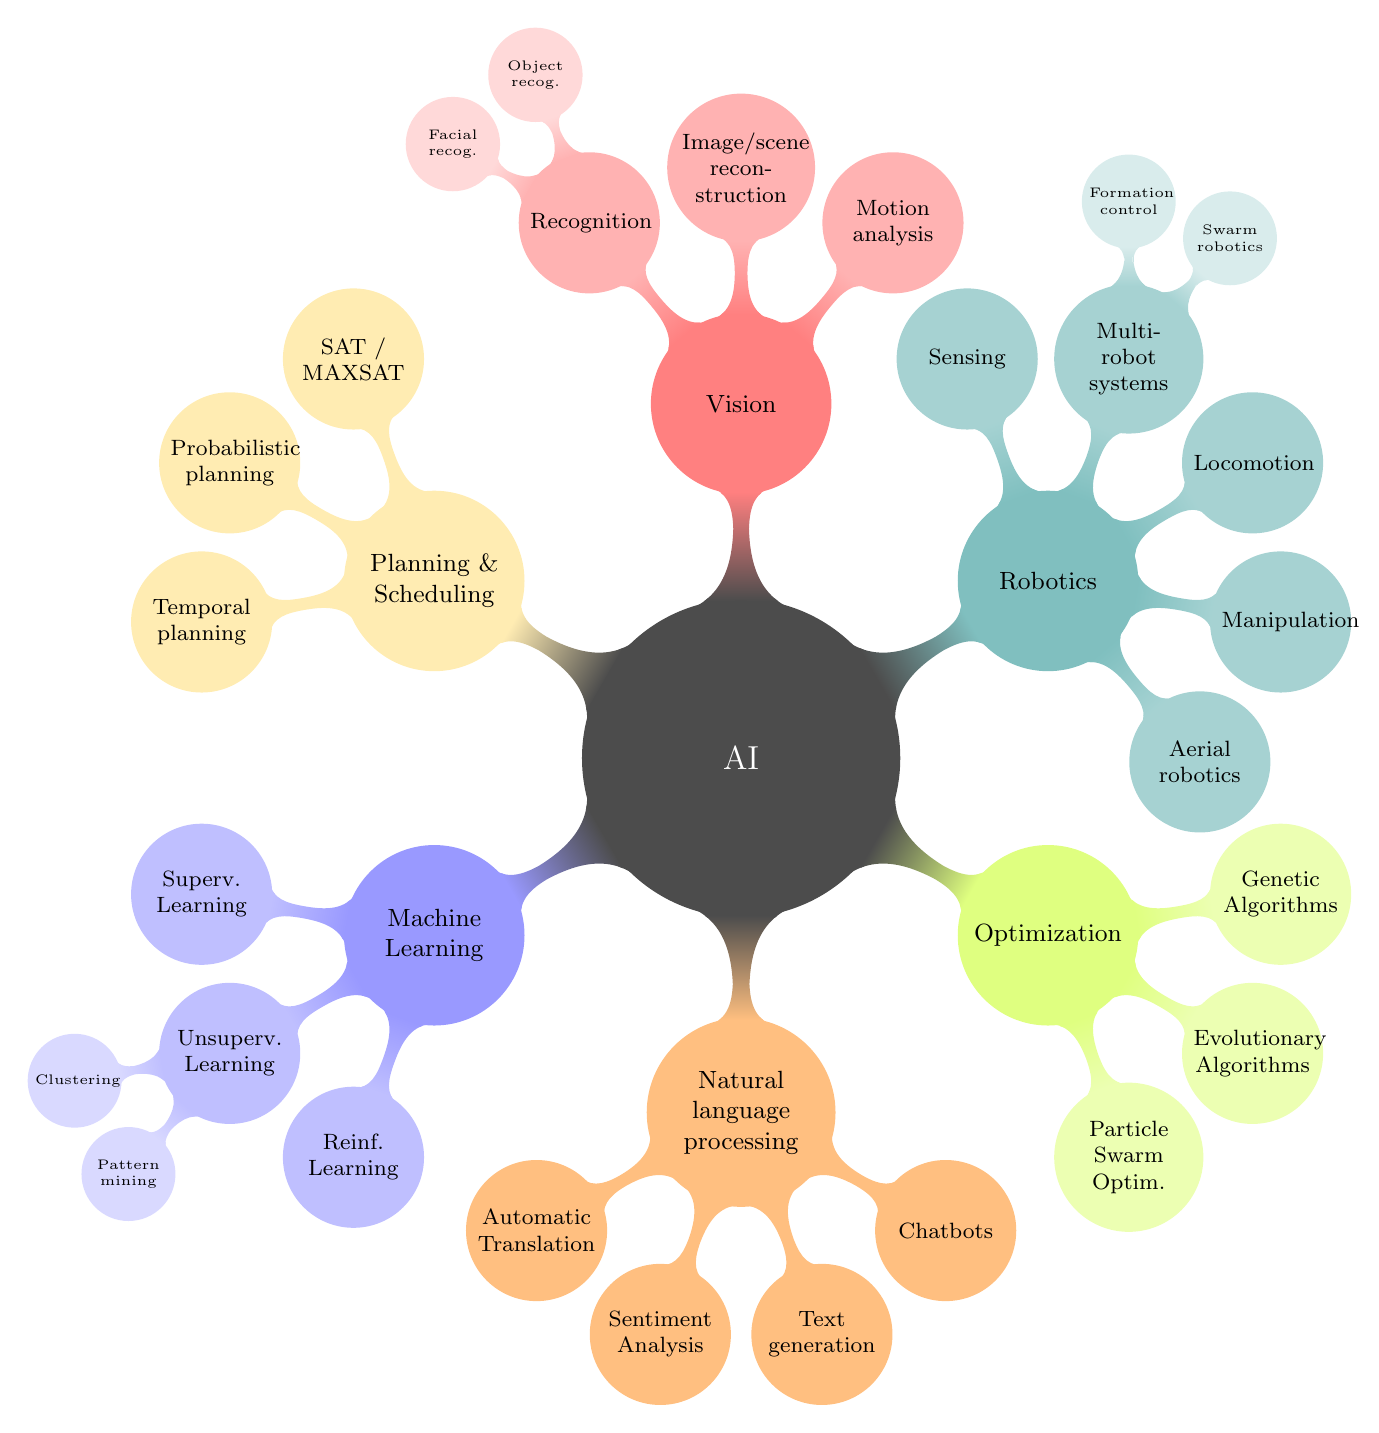
\begin{tikzpicture}[mindmap, grow cyclic, every node/.style=concept, concept color=black!70, text = white,
      level 1/.append style={level distance=4.5cm,sibling angle=60},
      level 2/.append style={level distance=3cm,sibling angle=40},
      level 3/.append style={level distance=2cm,sibling angle=40}]

      \node{AI}
      child [concept color=blue!40, text = black] { node {Machine Learning}
      child [concept color=blue!25]{ node {Superv. Learning}}
      child [concept color=blue!25]{ node {Unsuperv. Learning}
      child [concept color=blue!15]{ node {Clustering}}
      child [concept color=blue!15]{ node {Pattern mining}}
      }
      child [concept color=blue!25]{ node {Reinf. Learning}}
      }
      child [concept color=orange!50, text = black] { node {Natural language processing}
      child { node {Automatic Translation}}
      child { node {Sentiment Analysis}}
      child { node {Text generation}}
      child { node {Chatbots}}
      }
      child [concept color=lime!50, text = black] { node {Optimization}
      child [concept color=lime!30]{ node {Particle Swarm Optim.}}
      child [concept color=lime!30]{ node {Evolutionary Algorithms}}
      child [concept color=lime!30]{ node {Genetic Algorithms}}
      }
      child [concept color=teal!50, text = black] { node {Robotics}
      child [concept color=teal!35]{ node {Aerial robotics}}
      child [concept color=teal!35]{ node {Manipulation}}
      child [concept color=teal!35]{ node {Locomotion}}
      child [concept color=teal!35]{ node {Multi-robot systems}
      child [concept color=teal!15]{ node {Swarm robotics}}
      child [concept color=teal!15]{ node {Formation control}}
      }
      child [concept color=teal!35]{ node {Sensing}}
      }
      child [concept color=red!50, text = black] { node {Vision}
      child [concept color=red!30]{ node {Motion analysis}}
      child [concept color=red!30]{ node {Image/scene reconstruction}}
      child [concept color=red!30]{ node {Recognition}
      child [concept color=red!15]{ node {Object recog.}}
      child [concept color=red!15]{ node {Facial recog.}}
      }
      }
      child [concept color=amber!30, text = black] { node {Planning \& Scheduling}
      child { node {SAT / MAXSAT}}
      child { node {Probabilistic planning}}
      child { node {Temporal planning}}
      };
    \end{tikzpicture}%
    }
    \caption[AI Sub-Specialists]{\textit{AI Sub-Specialists. Note that these subfields often intersect and combine. }}
    {\label{fig:ai_branches}}
\end{figure}

\newpage

\section{Machine Learning}

Machine learning (ML) is a branch of artificial intelligence (\textit{AI}) and
computer science which focuses on the use of data and algorithms to imitate the
way that humans learn, gradually improving its accuracy
\cite{IBMMachineLearning}. \\

The central idea of machine learning is the existence of a mathematical
relationship between any combination of input and output data. Rather than
manually programming knowledge into computers, machine learning endeavors to
automatically learn significant relationships and patterns by observing
examples. \\

There are three subcategories (Figure \ref{fig:ml_branches}) of
machine learning \cite{MITML}.

\begin{itemize}
  \item \textbf{Supervised Learning}

    Machine learning models are trained with labeled data sets, which allow
    the models to learn and grow more accurate over time. For example, an
    algorithm would be trained with pictures of dogs and other things, all
    labeled by humans, and the machine would learn ways to identify pictures
    of dogs on its own. Supervised machine learning is the most common type
    used today.

  \item \textbf{Unsupervised Learning}

    Unsupervised learning involves using a training set that comprises
    unlabeled inputs, meaning inputs that do not have any assigned desired
    output. The primary objective of this learning approach is to uncover
    concealed patterns or data clusters without relying on human
    intervention.

  \item \textbf{Reinforcement Learning}

    Reinforcement learning occupies a position between supervised and
    unsupervised learning. In a certain sense, there is some form of
    supervision, but it does not involve explicitly specifying a desired
    output for every input in the data. Instead, a reinforcement learning
    algorithm receives feedback from the environment only after selecting an
    output, known as an action, based on a given input or observation. The
    feedback indicates the extent to which the action fulfills the learner's
    goals.

\end{itemize}

\newpage

\begin{figure}[H]
  \centering
  \resizebox{0.6\textwidth}{!}{%
    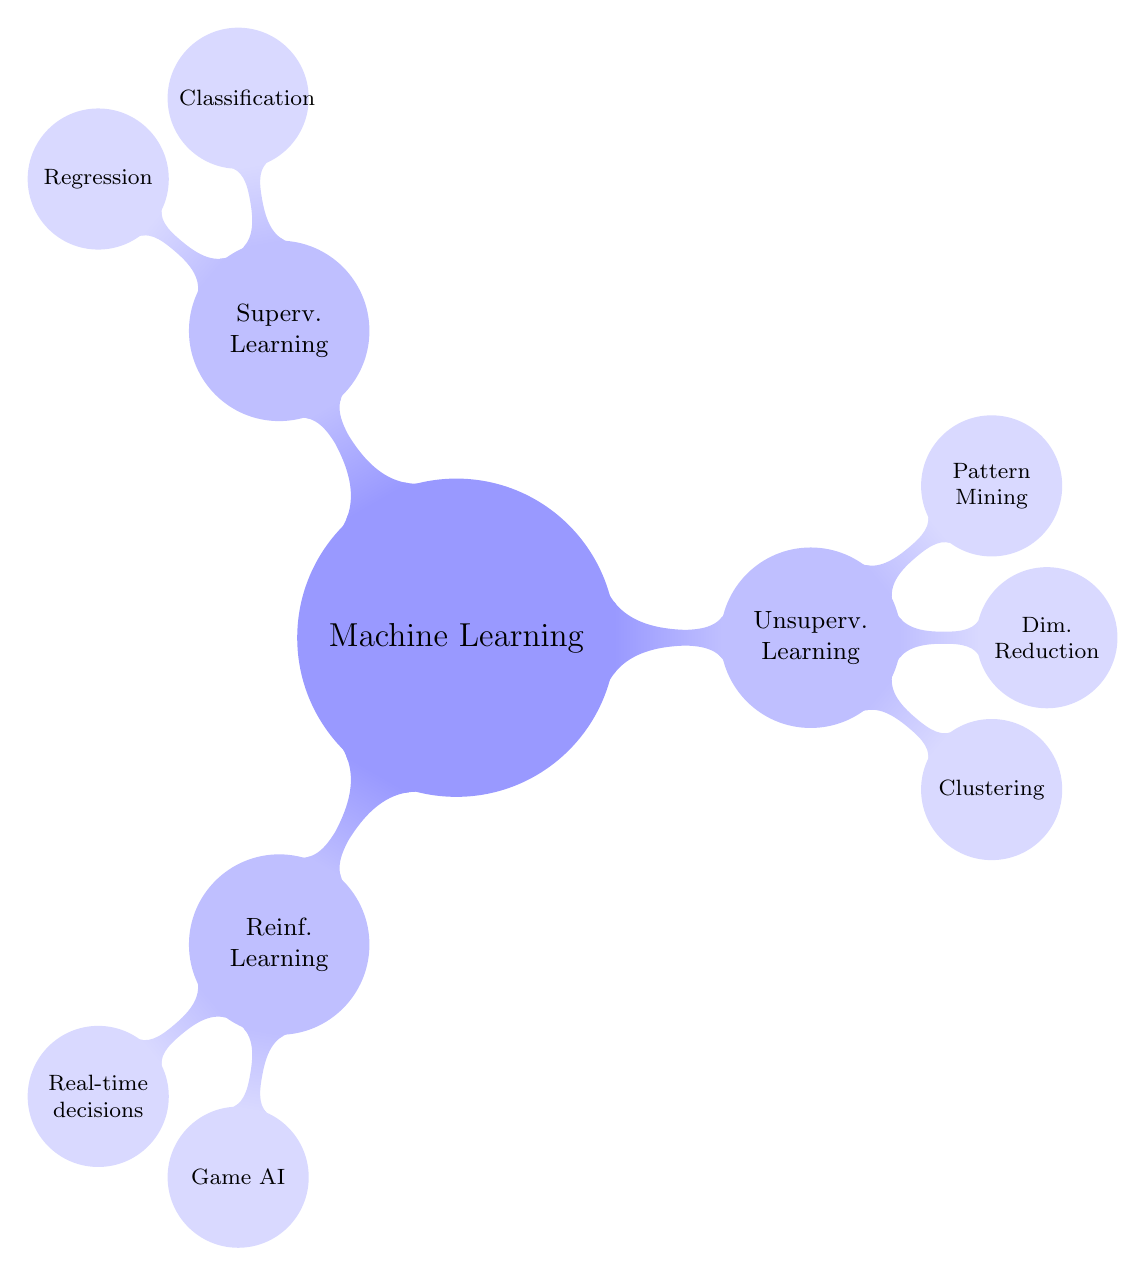
\begin{tikzpicture}[mindmap, grow cyclic, every node/.style=concept, concept color=blue!40, text = black,
      level 1/.append style={level distance=4.5cm,sibling angle=120},
      level 2/.append style={level distance=3cm,sibling angle=40},
      level 3/.append style={level distance=2cm,sibling angle=40}]

      \node{Machine Learning}
      child [concept color=blue!25, text = black] { node {Reinf. Learning}
      child [concept color=blue!15]{ node {Real-time decisions}}
      child [concept color=blue!15]{ node {Game AI}}
      }
      child [concept color=blue!25, text = black] { node {Unsuperv. Learning}
      child [concept color=blue!15]{ node {Clustering}}
      child [concept color=blue!15]{ node {Dim. Reduction}}
      child [concept color=blue!15]{ node {Pattern Mining}}
      }
      child [concept color=blue!25, text = black] { node {Superv. Learning}
      child [concept color=blue!15]{ node {Classification}}
      child [concept color=blue!15]{ node {Regression}}
      };
    \end{tikzpicture}%
    }
    \caption[Subcategories of Machine Learning.]{\textit{Subcategories of Machine Learning. }}
    {\label{fig:ml_branches}}
\end{figure}


\section{Deep Learning}

Deep learning, a subset of machine learning algorithms (Figure
\ref{fig:deep-learning-family}), is primarily associated with supervised
learning techniques. These algorithms derive conclusions by analyzing data with
a given logical structure. In contrast to traditional machine learning
algorithms, deep learning algorithms operate at a higher level of abstraction.
They possess the ability to perform the laborious process of feature
extraction. Each algorithm applies a nonlinear transformation to its input and
uses the acquired knowledge to generate a statistical model as the output. This
iterative process continues until the output reaches an acceptable level of
accuracy. The term "deep" refers to the number of layers the data must pass
through during these iterations. \\


Deep learning has been successfully applied to various problems, ranging from
self-driving cars to speech recognition. In this particular project, deep
learning is employed to classify whether a given dermoscopy image is a melanoma
or not. To achieve this, it has been necessary to understand how convolutional
neural networks work, address certain issues that affect the precision of these
models, explain the key metrics primarily used to measure the accuracy of these
models.

\newpage

\begin{figure}[H]
  \centering
  \includegraphics[width=0.6\textwidth]{imatges/preliminaries/deep-learning-family.jpg}
  \caption[Deep Learning Family]{\textit{Deep Learning Family. Illustration by Medium}}
  {\label{fig:deep-learning-family}}
\end{figure}

\section{Deep Neural Networks}

Deep neural networks are part of the deep learning algorithms within the realm
of machine learning, which, as mentioned earlier, falls under the umbrella of
artificial intelligence. is an
illustration of the deep learning family. \\


Deep neural networks, also known as fully connected layers (Figure
\ref{fig:deep-nn}), are modeled after the human brain. These algorithms achieve
their functionality by propagating signals from the input layer to the output
layer while passing through intermediate hidden layers. Each layer consists of
neurons responsible for detecting patterns from the incoming connections. These
neurons perform a crucial task by combining input from the data with a
corresponding set of coefficients, also known as weights. These weights act as
amplifiers or dampeners, modulating the impact of the input on the neuron's
activation. \\

By leveraging this mechanism, each layer in the deep neural network acquires
the capability to capture distinctive features from the input data. Notably, as
the signal travels deeper into the network, the extracted features become
increasingly sophisticated and abstract. This characteristic arises from the
hierarchical nature of the network architecture, enabling the model to learn
and discern intricate patterns and representations. \\

The process of feature extraction in deep neural networks allows the network to
progressively learn and uncover complex relationships within the data. As the
signal traverses through the network's layers, each subsequent layer builds
upon the extracted features from the previous layer, resulting in the
generation of more intricate and comprehensive representations. This ability to
capture and model hierarchical features is a significant advantage of deep
neural networks, making them particularly effective in tasks requiring the
recognition of complex patterns and high-level abstractions.

\begin{figure}[H]
  \centering
  \includegraphics[width=0.6\textwidth]{imatges/preliminaries/deepnn.jpg}
  \caption[Deep Neural Network] {\textit{Deep Neural Network.
  Illustration by Medium}}
  {\label{fig:deep-nn}}
\end{figure}

The minimum unit in a layer is known as a perceptron or neuron, which bears a
resemblance to human neurons (Figure \ref{fig:perceptron}). The perceptron was
created by Frank Rosenblatt in 1958 and it is the oldest form of a simple
neural network. \\

Each perceptron in the network has an associated value that is computed based
on the incoming nodes and edges. The computation occurs as follows: the
products of inputs and their respective weights are summed with a bias, and
this sum then passes through the node's activation function. The purpose of the
activation function is to compress the resulting value within the range of 0 to
1, introducing non-linearity and enabling the model to learn complex
relationships within the data. The resultant value determines the extent to
which the signal should propagate through the network, thus influencing the
final outcome.


\begin{figure}[H]
  \centering
  \includegraphics[width=0.8\textwidth]{imatges/preliminaries/perceptron.png}
  \caption[The Perceptron]{\textit{The Perceptron. Illustration by Medium}}
  {\label{fig:perceptron}}
\end{figure}

\newpage

\section{Convolutional Neural Networks}

A convolutional neural network (CNN) is a specific type of neural network that
is particularly well suited for analyzing images. One of the key innovations of
CNNs is their ability to automatically learn a large number of filters in
parallel. These filters are learned during the training process and are
specifically tailored to solve a particular predictive modeling problem, such
as image classification. By learning these filters, CNNs become adept at
extracting relevant features and patterns from visual data without the need for
manual feature engineering. \\

CNNs are designed to learn spatial hierarchies of features through a process
called back-propagation. During training, the network adapts its internal
parameters, or weights, by iteratively propagating the error backwards from the
output to the input layers. This allows the network to gradually adjust its
weights in a way that minimizes the difference between its predicted outputs
and the true outputs. \\

One key distinction of CNNs compared to regular neural networks is their use of
parameter sharing. In a CNN, all neurons within a particular feature map share
the same weights. This sharing of weights significantly reduces the number of
parameters in the network, making it more computationally efficient. By sharing
weights, the network can detect the same patterns or features regardless of
their spatial position in the input data. This property, known as translation
invariance, enables CNNs to recognize objects or patterns regardless of their
location within an image.\\

To build a CNN, we need four main types of layers:

\begin{itemize}
  \item Convolutional Layers
  \item Pooling Layers
  \item Fully Connected Layers
  \item Non-linearity Layers
\end{itemize}

\subsection{Convolutional Layers}

A convolutional layer (Figure \ref{fig:convolutional-layer}) is
responsible for detecting and extracting features from the input data. It
consists of a set of learnable filters, also known as kernels or feature
detectors. Each filter is a small matrix of weights that convolves
across the input data to perform a dot product operation at each spatial
location.  \\

The filter convolves across the input data with a defined stride,
which specifies the amount of shift between each position. At each spatial
location, a dot product is computed between the filter and the overlapping
region of the input. The dot product involves element-wise multiplication of
the filter values with the corresponding input values, followed by summing up
the results. \\

The result of each dot product operation is a single value, forming a pixel in
the output feature map. Additionally, an activation function is applied
element-wise to introduce non-linearity into the network.

\begin{figure}[H] \centering
  \begin{adjustbox}{width=0.75\textwidth, trim={0cm 0cm 0cm 0.35cm}, clip}
  \includegraphics[]{imatges/preliminaries/convolutional-layer.png}
  \end{adjustbox}
  \caption[Convolutional Operation on Input]{\textit{Convolutional
  Operation on Input. Illustration by towardsdatascience}}
{\label{fig:convolutional-layer}} \end{figure}

\newpage

\subsection{Pooling Layers}

A pooling layer (Figure \ref{fig:pooling-layer}) performs a
summarizing of nearby outputs in the network, effectively replacing certain
locations with a condensed representation. This reduces the spatial
dimensionality of the output, leading to decreased computational requirements
and weight parameters. The pooling operation is applied independently to each
slice of the representation. \\

Various pooling functions exist, including averaging the values within a
rectangular neighborhood, computing the L2 norm of the neighborhood, or using a
weighted average based on distance. However, the most widely used method is max
pooling, which selects the maximum output value from the neighborhood.

\begin{figure}[H]
  \centering
  \includegraphics[width=0.8\textwidth]{imatges/preliminaries/polling-layer.png}
  \caption[Max Polling Operation on Input]{\textit{Max Polling Operation on Input. Illustration by towardsdatascience}}
  {\label{fig:pooling-layer}}
\end{figure}

\subsection{Fully Connected Layers}

Neurons in this layer have full connectivity with all neurons in the preceding
and succeeding layer. This is why it can be computed as usual by a matrix
multiplication followed by a bias effect. The topology in the fully connected
portion of a CNN depends on various factors, including the complexity of the
task, the nature of the data, and the capacity of the model. There is no fixed
rule for determining the exact number of neurons or layers, and it often
requires experimentation and tuning. \\

A fully connected layer (Figure \ref{fig:deep-nn}), helps to map the
representation between the input and the output.

\subsection{Non-linearity Layers}

Convolutional operations in neural networks are linear, meaning they capture
linear patterns in the data. However, many objects in images exhibit non-linear
characteristics that cannot be effectively detected using linear operations
alone. To address this limitation, non-linearity layers, such as activation
functions, are typically applied immediately after the convolutional layer.
These non-linearity layers may introduce non-linear transformations to the
activation maps, enabling the network to learn and detect complex, non-linear
patterns in the data. \\

There are many types of non-linearity functions applied after the convolutional
layers, the most popular are: \\

\begin{itemize}

  \item \textbf{Sigmoid}

    The sigmoid function takes a real-valued number and “squashes” it into a
    range between 0 and 1.

    \centering {
      \begin{tikzpicture}
        \draw[->] (-5,0) -- (5,0) node[right] {$x$};
        \draw[->] (0,-0.5) -- (0,1.5) node[above] {$\sigma(x)$};
        \draw[domain=-5:5, smooth, variable=\x, blue] plot (\x, {1/(1 + exp(-\x))});
        \draw[dashed] (-5, 0.0) node[left] {0};
        \draw[dashed] (-5, 1) node[left] {1} -- (5, 1);
      \end{tikzpicture}
    }

    \raggedright
    Mathematically, the sigmoid function is expressed as:

    \[ \sigma(x) = \frac{1}{1 + e^{-x}} \]

    \newpage

  \item \textbf{ReLU}

    The Rectified Linear Unit (ReLU) is maybe the most popular activation
    functions in the last few years. The function is just simply threshold at
    zero.

    \centering \begin{tikzpicture} \draw[->] (-5,0) -- (5,0) node[right]
      {$x$}; \draw[->] (0,-0.5) -- (0,5) node[above] {$\text{ReLU}(x)$};
      \draw[domain=-5:0, smooth, variable=\x, blue] plot (\x, 0);
      \draw[domain=0:5, smooth, variable=\x, blue] plot (\x, \x);
      \draw[dashed] (-5, 0.0) node[left] {0}; \draw[dashed] (-5, 1) node[left]
    {1} -- (5, 1); \end{tikzpicture}

    \raggedright
    Mathematically, the ReLU function is expressed as:

    \[f(x) = \max(0, x)\]

  \item \textbf{Tanh}

    The hyperbolic tangent function tanh compresses a real-valued number to
    the range of [-1, 1]. Similar to the sigmoid function, tanh exhibits
    saturation, but unlike sigmoid, its output is centered around zero.

    \centering
    \begin{tikzpicture}
      \draw[->] (-5,0) -- (5,0) node[right] {$x$};
      \draw[->] (0,-1.5) -- (0,1.5) node[above] {$\tanh(x)$};
      \draw[domain=-5:5, smooth, variable=\x, blue] plot (\x, {tanh(\x)});
      \draw[dashed] (-5, -1) node[left] {-1} -- (5, -1);
      \draw[dashed] (-5, 1) node[left] {1} -- (5, 1);
    \end{tikzpicture}

    \raggedright
    Mathematically, the tanh function is expressed as:

    \[ \tanh(x) = \frac{{e^x - e^{-x}}}{{e^x + e^{-x}}} \]

\end{itemize}

\section{Loss Function}

A loss function, also known as a cost function or an objective function, is a
measure used in machine learning and optimization algorithms to quantify how
well a model performs on a given task. It measures the discrepancy between
the predicted outputs of a model and the true values or labels associated with
the training data. \\

Different machine learning tasks and algorithms may use different loss
functions, depending on the specific problem being addressed. Commonly used
loss functions include:

\begin{itemize}
  \item Mean Squared Error (MSE)
  \item Binary Cross-Entropy
  \item Mean Absolute Error (MAE)
  \item Cross-entropy Loss
\end{itemize}

For this thesis, the loss function used to train the models is
Cross-entropy Loss as this is a multiclass problem. Do not confuse the
optimizer algorithm with the metric used to evaluate how good models are. We
used the ROC AUC with one-vs-rest strategy to evaluate the models performance,
explained in Section \ref{sec:metrics}. \\

Cross-entropy loss, also known as log loss, is a widely used loss function in
machine learning, particularly in classification tasks. It measures the
dissimilarity between predicted class probabilities and true class labels.
\\

In multi-class classification, the cross-entropy loss is calculated using the
true class labels \(y\) and the predicted class probabilities \(p\) for each
class. It can be defined as:

\[-\sum_{i=1}^{C} y_i \log(p_i)\]

\noindent where:

\begin{itemize}
  \item \(C\) is the total number of classes.
  \item \(y_i\) represents the true label for class \(i\).
  \item \(p_i\) represents the predicted probability for class \(i\).
\end{itemize}

\section{Metrics}
{\label{sec:metrics}}

There are various metrics commonly used to assess the quality of a model's predictions.
In this section, we present a selection of metrics that we find relevant for evaluating our models.

\subsection{Confusion Matrix}

A confusion matrix (Figure \ref{fig:confusion-matrix}) is a square matrix with dimensions  NxN,
where  N represents the total number of classes being predicted.
It provides a visual representation of the errors or confusion made by a classification
model during its predictions. \\


\begin{figure}[H]
  \begin{adjustbox}{trim={0pt 0.5cm 0pt 1cm}, clip}
    \centering
    \includegraphics[width=0.9\textwidth]{imatges/preliminaries/confusion-matrix.png}
  \end{adjustbox}
  \caption[Confusion Matrix Multi-Class]{\textit{Confusion Matrix Multi-Class. Illustration by kaggle}}
  {\label{fig:confusion-matrix}}
\end{figure}

From confusion matrix we can obtain other metrics such as:

\begin{itemize}
  \item \textbf{True Positive (TP)}

    This refers to an outcome where the model accurately predicts the positive class.
  \item \textbf{False Positive (FP)}

    This describes a situation where the model mistakenly predicts the positive class when it should have predicted the negative class.
  \item \textbf{True Negative (TN)}

    This represents an outcome where the model correctly predicts the negative class.
  \item \textbf{False Negative (FN)}

    This indicates a scenario where the model incorrectly predicts the negative class instead of predicting the positive class.

\end{itemize}


In a logical sense, when we add up the elements on the main diagonal of the
confusion matrix, we obtain the total number of correct predictions.
Utilizing the confusion matrix values, we can compute
additional metrics such as accuracy, recall and others.

\subsection{Accuracy}

Accuracy is a commonly employed and straightforward performance metric in
classification tasks. It calculates the ratio of correct predictions to the
total number of predictions made on a dataset, thus determining the likelihood
of correctly classifying an input. Accuracy is especially valuable when working
with a balanced dataset, where the number of instances in each class is roughly
equivalent.

\[Accuracy = \frac{TP + TN}{TP + TN + FP + FN}\]

\subsection{TPR}

TPR stands for True Positive Rate, and it is also known as sensitivity or
recall. It measures the proportion of actual positive cases that are correctly
identified as positive by a classification model or test.

\[
  \text{TPR} = \frac{\text{TP}}{\text{TP} + \text{FN}}
\]

\subsection{FPR or Recall}

FPR stands for False Positive Rate, and it measures the proportion of actual
negative cases that are incorrectly identified as positive by a classification
model or test.

\[ \text{FPR} = \frac{\text{FP}}{\text{FP} + \text{TN}} \]

\subsection{AUC-ROC}

The ROC Curve, when computed with the one-vs-rest (OvR) strategy for
multi-class classification, provides insights into how well the model can
differentiate a class from the rest of the classes. It is a probabilistic curve
that plots the true positive rate (TPR) against the false positive rate (FPR).
By treating the target class as the positive class and the remaining classes as
the negative class in separate binary classification tasks (\textit{Figure
\ref{fig:auc-roc}}). \\

The area under the curve (AUC) is a value between 0 and 1 that measures the
ability of a classifier to distinguish between classes. It is used as a summary
of the ROC curve. The higher the AUC, the better the performance of the model
at distinguishing between the positive and negative classes.

\begin{figure}[H]
  \centering
  \includegraphics[width=0.7\textwidth]{imatges/preliminaries/auc.png}
  \caption[AUC-ROC Performance]{\textit{AUC-ROC Performance. Illustration by Elizabeth Louise Thomas}}
  {\label{fig:auc-roc}}
\end{figure}

\newpage

\section{Optimizer}

An optimizer is an algorithm that finds the value of the parameters (weights)
that minimize the error when mapping inputs to outputs. While training a deep
learning models, the optimizer modifies the weights of the model in each epoch
to minimize the loss function. \\

The are a considerable amount of different optimizer algorithms out there with
their pros and cons. In this section we present the family of optimizers based
on Gradient Descent optimization. This family of optimizer algorithms were used
for the thesis. \\

\subsection{Gradient Descent}

Using the Gradient Decent (SD) optimization algorithm (Figure
\ref{fig:optimization}), the weights are updated incrementally after each
epoch. The magnitude and direction of the weight update is computed by taking a
step in the opposite direction of the cost gradient. \\

Given the following defintions:

\begin{itemize}
  \item \(\Delta w\) represents the weights update.
  \item \(\eta\) (eta) denotes the "learning rate", which controls the step size of the update.
  \item  \(\frac{\partial J}{\partial w_i}\) represents the partial derivative of the cost function \(J\) with respect to the weight \(w_i\).
  \item \(\nabla J(w)\) represents the gradient of the cost function \(J(w)\) with respect to the weights \(w\).
\end{itemize}

We could compute the weight update after each epoch with the following
mathematical expression:

\[\nabla J(w) = (\frac{\partial J}{\partial w_1}, \frac{\partial J}{\partial w_2}, \ldots, \frac{\partial J}{\partial w_n})\]

\[
  \Delta w = -\eta \cdot \nabla J(w)
\]


\[
  w = w + \Delta w
\]



In Gradient Descent optimization, we compute the cost gradient based on the
complete training set, in case of very large datasets, using Gradient Descent
can be quite costly since we are only taking a single step for one pass over
the training set – thus, the larger the training set, the slower our algorithm
updates the weights and the longer it may take until it converges to the global
cost minimum. \\

A high level pseudo-implementation of the Gradient Descent algorithm: \\

\begin{itemize}[label=\(\circ\)]
  \item for each epoch:
    \begin{itemize}[label=\(\circ\), topsep=0pt]
      \item for each weight \(j\):
        \begin{itemize}[label=\(\circ\), topsep=5pt]
          \item \(w_j = w_{j-1} + \Delta w_j\)
        \end{itemize}
    \end{itemize}
\end{itemize}

\begin{figure}[H]
  \centering
  \includegraphics[width=0.5\textwidth]{imatges/preliminaries/optimization.png}
  \caption[Optimization Using Gradient Descent]{\textit{Optimization Using Gradient Descent. Illustration by raschka}}
  {\label{fig:optimization}}
\end{figure}

\newpage

\subsection{Stochastic Gradient Descent}

Stochastic Gradient Descent (SGD) work similar to the Gradient Descent but the
weight updates are not accumulated as we have seen above for Gradient Descent.
Instead, the weights are updated after each training sample. Due to its
stochastic nature, the path towards the global cost minimum is not “direct” as
in Gradient Descent, but may go “zig-zag”if we are visualizing the cost surface
in a 2D space, see Figure \ref{fig:sgdvsgd}. However, it has been shown that
Stochastic Gradient Descent almost surely converges to the global cost minimum
if the cost function is convex. \\

A high level pseudo-implementation of the Stochastic Gradient Descent
algorithm:

\begin{itemize}[label=$\circ$]
  \item for each epoch or until approx. cost minimum is reached:
    \begin{itemize}[label=$\circ$, topsep=0pt]
      \item for training sample \(i\):
        \begin{itemize}[label=$\circ$, topsep=5pt]
          \item for each weight \(j\):
            \begin{itemize}[label=$\circ$, topsep=10pt]
              \item \(w_j = w_{j-1} + \Delta w_j\), where \(\Delta w_j = \eta (target^{(i)} - output^{(i)})x_{j}^{(i)}\)
            \end{itemize}
        \end{itemize}
    \end{itemize}
\end{itemize}

\begin{figure}[H]
  \centering
    \includegraphics[width=0.8\textwidth]{imatges/preliminaries/sgdvsgd.jpeg}
  \caption[GD vs SGD]{\textit{GD vs SGD. Illustration by superannotate}}
  {\label{fig:sgdvsgd}}
\end{figure}

\newpage

\section{Forward and Backward Propagation}

Forward and back-propagation are fundamental processes in training neural
networks and optimizing their parameters. They play a crucial role in enabling
the network to learn from data and improve its performance over time. \\

Resuming the forward-propagation and back-propagation (\textit{Figure
\ref{fig:forward-and-back-propagation}}), in order to find the direction of the
steepest descent (minimising the overall loss function), we need to calculate
gradients of the loss function with respect to weights and bias. After that,
we’ll be able to update weights and bias using negative gradients multiplied by
the learning rate.

\begin{figure}[H]
  \centering
  \includegraphics[width=0.8\textwidth]{imatges/preliminaries/front-and-back-prop.png}
  \caption[Forward and Backward Propagation]{\textit{Forward and Backward Propagation. Illustration by baeldung}}
  {\label{fig:forward-and-back-propagation}}
\end{figure}


\subsection{Forward Propagation}

Forward propagation refers to the process of computing the output of a neural
network given an input or a batch of inputs. During forward propagation, the
input data flows through the network's layers in a sequential manner, from the
input layer to the output layer. Each layer performs a series of computations,
typically involving linear transformations (such as matrix multiplications)
followed by activation functions. \\

As the data flows forward through the network, intermediate outputs, also known
as activations or feature maps, are computed at each layer. These activations
are then passed on as inputs to the subsequent layers until the final output is
produced. The forward propagation process essentially calculates the predicted
output of the network for a given input.

\subsection{Backward Propagation}

Backward propagation, short for backward propagation of errors, is the process
of computing the gradients of the network's parameters with respect to a loss
function. These gradients indicate the sensitivity of the network's output to
changes in its parameters and are used to update the parameters during the
training process. \\

The backward propagation algorithm starts from the final output of the network
and propagates the error gradients backward through the network's layers. It
computes the gradients layer by layer using the chain rule of calculus. The
gradients quantify how each parameter contributed to the overall error of the
network and provide information on how to adjust the parameters to reduce the
error.


\section{Under-fitting vs Over-fitting}

Under-fitting is a prevalent challenge in machine learning, occurring when the
model fails to establish a meaningful relationship between the input and target
variable. Insufficiently capturing the features of the data results in
increased errors in both the training and unseen data samples. \\

Over-fitting is also a prevalent challenge in machine learning but it is really
common in deep learning algorithms. Deep learning models try to fit the
training data entirely and ends up memorizing the data patterns and the
noise/random fluctuations. These models fail to generalize and perform well in
the case of training data, but fail in unseen data scenarios, defeating the
model's purpose.

\begin{figure}[H]
  \centering
  \begin{adjustbox}{width=\textwidth, trim={0cm 1.25cm 0cm 2.25cm}, clip}
  \includegraphics[width=\textwidth]{imatges/preliminaries/fit-scenes.jpg}
  \end{adjustbox}
  \caption[Fitting Scenarios]{\textit{Fitting Scenarios. Illustration by towardsdatascience}}
  {\label{fig:underfitting-overfitting-goodfitting}}
\end{figure}

\section{Strategies to Combat Over-fitting}

There are lot of strategies to combat over-fitting, in this section there is
presented only those used in the project. \\

\subsection{Early Stopping}

Early Stopping involves monitoring the model's performance on a validation
dataset during training. If the performance stops improving or starts
deteriorating, the training process is stopped early. By doing this, early
stopping helps find the optimal balance between model complexity and
generalization, ensuring the model does not become overly specialized to the
training data and does not perform well on unseen data. \\

\begin{figure}[H]
  \centering
  \includegraphics[width=0.7\textwidth]{imatges/preliminaries/early-stop.png}
  \caption[Early Stopping]{\textit{Early Stopping. the vertical doted line
  represents the point where the early stop mechanism should have been
  triggered. Illustration by wandb}}
  {\label{fig:early-stop}}
\end{figure}

\subsection{Learning Rate Scheduling}

The learning rate is a hyper-parameter in machine learning that determines the
step size at which a model's parameters are updated during the optimization
process. In most optimization algorithms, such as gradient descent, the
learning rate controls how quickly or slowly the model learns from the training
data. \\

There are various approaches in learning rate scheduling, below you will find
the scheduling used in the thesis.

\begin{itemize}
  \item \textbf{Learning Rate Decay}

    This learning rate scheduling works gradually reducing the learning rate
    over time or in response to certain conditions. \\

    A smaller learning rate allows the model to fine-tune its parameters more
    cautiously, preventing it from aggressively fitting to noisy or
    irrelevant patterns in the training data. A smoother or an agresive
    adjustment helps the model converge to a better generalized solution,
    reducing the risk of over-fitting. \\

    There are varius scheduler policies that we can follow to make the
    learning rate decay over the epochs. For instance, in Figure
    \ref{fig:learning-rate-decay-cosine-annealing} follows the
    Cosine Annealing Learning Rate scheduler, yet Figure
    \ref{fig:learning-rate-decay-step} follows the Step Learning
    Rate scheduler.

    \begin{figure}[H] \centering
      \includegraphics[width=0.6\textwidth]{imatges/preliminaries/cosinus-scheduler.png}
      \caption[Cosine Annealing Learning Rate Scheduler]{\textit{Cosine
      Annealing Learning Rate Scheduler. A learning rate decay scheduler with
      smoother behavior. }}
    {\label{fig:learning-rate-decay-cosine-annealing}} \end{figure}

    \begin{figure}[H] \centering
      \includegraphics[width=0.6\textwidth]{imatges/preliminaries/step-scheduler.png}
      \caption[Step Learning Rate Scheduler]{\textit{Step Learning Rate
      Scheduler. A learning rate decay scheduler with and agresive behavior.
      }} {\label{fig:learning-rate-decay-step}}
    \end{figure}

    \newpage

  \item \textbf{Cycling Learning}

    Cyclic learning rate scheduling is popular for faster convergence and
    improved generalization. By cycling the learning rate, models explore
    diverse loss landscape regions, escaping local minima for better optima.
    Variations like triangular and cosine annealing alternate or smoothly
    transition between lower and upper bounds. This approach adds variation
    and exploration to optimization, enhancing model performance and
    convergence. \\

    As well as in learning rate decay, there are various scheduler with it's
    own policy. Figure \ref{fig:cycling-rate-decay} is a
    representation of a Cosine Annealing Warm Restart scheduler.
    \begin{figure}[H] \centering
      \includegraphics[width=0.6\textwidth]{imatges/preliminaries/CosineAnnealingWarmRestarts-scheduler.png}
      \caption[Cosine Annealing Warm Restart]{\textit{Cosine Annealing Warm
      Restart. A cosinus cycling learning scheduler.}}
    {\label{fig:cycling-rate-decay}} \end{figure} \end{itemize}

\newpage

\subsection{Dropout}

Dropout is a regularization method \cite{DropoutPaper}. The idea behind dropout
is to prevent over-fitting and improve generalization in neural networks by
randomly "dropping out" or deactivating a fraction of the neurons during
each training iteration. \\

By randomly dropping out neurons, the network becomes more robust and less
sensitive to the precise configuration of any single neuron. It forces the
network to learn redundant representations and prevents co-adaptation.

\begin{figure}[H]
  \centering
  \includegraphics[width=10cm]{imatges/preliminaries/dropout.png}
  \caption[Dropout]{\textit{Dropout Neural Net Model. \textbf{Left}: A standard neural net with 2 hidden layers. \textbf{Right}:
  An example of a thinned net produced by applying dropout to the network on the left.
  Crossed units have been dropped. Illustration by Srivastava}}
  {\label{fig:dropout}}
\end{figure}

\newpage

\subsection{Data Augmentation}

Data augmentation encompasses various techniques utilized to expand the dataset
by introducing modifications, thereby increasing the number of examples. Its
purpose is not only to enlarge the dataset but also to enhance its diversity.
By acting as a regularization, data augmentation aids in mitigating
over-fitting during machine learning model training.

\begin{figure}[H]
  \centering
  \includegraphics[width=0.7\textwidth]{imatges/preliminaries/augmentation.jpg}
  \caption[Data Augmentation]{\textit{Data Augmentation. Illustration by Albumentations}}
  {\label{fig:augmentation}}
\end{figure}


\section{Train, Validation and Test Sets}

The primary method employed to validate the models involves dividing the
original dataset into three subsets using the Holdout set scheme (Figure
\ref{fig:holdout-test-scheme}).

\begin{figure}[H]
  \centering
  \begin{adjustbox}{width=0.8\textwidth, trim={0cm 0.5cm 0cm 0.5cm}, clip}
    \includegraphics[width=\textwidth]{imatges/preliminaries/train-test-validation-sets.png}
  \end{adjustbox}
  \caption[Holdout Set Scheme]{\textit{Holdout Set Scheme. Illustration by Qualcomm}}
  {\label{fig:holdout-test-scheme}}
\end{figure}

The Holdout set scheme involves dividing the data into two sets: one for
training and another for testing. Additionally, a validation set is created
from the training set to assess how well the model performs on unseen data
during training. \\

During the training phase, the test set remains completely separate and is not
used in any way to configure the hyper-parameters. This ensures that the
model's performance on the validation set is not artificially inflated by
adjusting hyper-parameters to achieve an exceptionally good outcome. \\

The data from the ISIC Archive was divided using the following percentages: 80%
for training, 10\% for validation, and 10\% for testing.

\section{Test-Time Augmentation}

Test-time augmentation (TTA) is used during the testing or inference phase of a
machine learning model. TTA generates multiple augmented versions of test
samples to obtain diverse predictions. By obtaining predictions from these
augmented samples and combining them, TTA mimics the behavior of an ensemble of
models.

\begin{figure}[H]
  \centering
  \includegraphics[width=0.8\textwidth]{imatges/preliminaries/tta.png}
  \caption[Test-Time Augmentation]{\textit{Test-Time Augmentation. Illustration by stepup.ai}}
  {\label{fig:tta}}
\end{figure}

\newpage

\section{ResNet}

ResNet, short for "Residual Network," is a deep convolutional neural network
(CNN) architecture that was introduced in 2015 by researchers from Microsoft
Research \cite{ResNetPaper}. It revolutionized the field of deep learning by
addressing the challenge of training very deep neural networks. \\

The main problem encountered when training deep neural networks is the
degradation problem, where the accuracy of the model saturates and then starts
to decline rapidly as the network depth increases. This degradation occurs due
to the difficulty of optimizing the network's parameters and the vanishing
gradient problem, where gradients become extremely small during
backpropagation, making it difficult for the network to learn effectively.
\\

ResNet tackled this problem by introducing the concept of residual learning.
The key idea is to use "skip connections" or "identity mappings" that allow the
network to learn residual functions. Instead of trying to learn the underlying
mapping directly, ResNet models learn the residual between the desired mapping
and the input. \\

By introducing these skip connections, ResNet models can effectively "skip" one
or more layers during training, allowing information to flow more easily
through the network. This mitigates the degradation problem and enables the
training of extremely deep networks (e.g., hundreds of layers) without
suffering from diminishing accuracy. \\

In ResNet, each layer of the network contains a residual block. A residual
block consists of multiple convolutional layers followed by batch normalization
and activation functions. The input to a residual block is added to its output
through a skip connection, which directly connects the input to the output.
This allows the network to learn the residual information, or the difference
between the input and the desired output, making it easier for the network to
learn the underlying mapping.  \\

There are various architectural variants or "flavors" of ResNet, including
ResNet-152,  ResNet-101,  ResNet-50,  ResNet-34, and  ResNet-18. The
number following the name of each ResNet variant indicates the number of inner
layers present in the architecture.

\newpage

As evident from Figure \ref{fig:resnet}, it can be observed that
ResNet architectures with a greater number of layers tend to exhibit higher
accuracy. However, it is important to note that this improvement in accuracy
comes at the expense of having a significantly larger number of parameters to
train.


\begin{figure}[H]
  \begin{adjustbox}{width=\textwidth, trim={0pt 0pt 1cm 0pt}, clip}
    \centering
    \includegraphics[width=\textwidth]{imatges/preliminaries/ResNetImageNet.png}
  \end{adjustbox}
  \caption[ResNet "flavors" Results on ImageNet]{\textit{ResNet "flavors" Results on ImageNet. Illustration by paperswithcode}}
  {\label{fig:resnet}}
\end{figure}

To accurately assess the performance of each ResNet architecture, refer to
Table \ref{table:resnet}, which provides the accuracy achieved on the ImageNet
dataset along with the corresponding number of trainable parameters in
millions.

\begin{table}[H]
  \centering
  \begin{tabular}{lcc}
    \toprule
    \textbf{Model} & \textbf{Accuracy} & \textbf{Parameters} \\
    \midrule
    ResNet-152 & 78.31\% & 60.2M \\
    ResNet-101 & 77.37\% & 44.5M \\
    ResNet-50 & 76.15\% & 25.6M \\
    ResNet-34 & 73.30\% & 21.8M \\
    ResNet-18 & 69.76\% & 11.7M \\
    \bottomrule
  \end{tabular}
  \caption[Accuracy achieved on ImageNet and trainable parameters of each resNet.]
  {\textit{Accuracy achieved on ImageNet and trainable parameters of each resNet.
  Each image in the ImageNet dataset is associated with 1 of 1,000 classes. Table by paperswithcode}}
  {\label{table:resnet}}
\end{table}

\section{Micro-services Architecture}

A micro-services architecture is a software design approach that structures an
application as a collection of small, independent services, each running in its
own process and communicating with each other through lightweight mechanisms.
This architecture promotes scalability, modularity and flexibility. \\

As a result of this thesis we built two services: an API and a UI. These services
are built using different frameworks and programming languages.

\section{Inference API}

The inference API service focuses on handling the back-end logic and data
processing. It exposes a well-defined API that allows user to interact with the
trained models. \\

The end-points that the present thesis API service support are explained in
Section \ref{cap:result}.

\section{Containerization}

Containerization is a technology that allows applications and their
dependencies to be packaged into isolated, lightweight containers. These
containers provide an encapsulated runtime environment, ensuring that the
application runs consistently across different systems. \\

Containers are created from container images, which are self-contained packages
containing the application's code, dependencies, libraries, and configurations.
Images serve as the blueprint for creating containers. They can be shared,
versioned, and easily deployed on various platforms. \\

Frameworks such as Docker and Podman, provide tools and services to build,
manage, and run containers. These frameworks utilize underlying virtualization
technologies to create and manage isolated environments. These environments,
called containers, offer resource isolation and ensure that applications run
consistently across different computing environments. As a result, services
running in containers are easy to maintain, portable and fast to start-up.

\section{Platform Deployment}

To distribute the containerized API and UI services easily to professionals,
there are several solutions available. In this thesis, we propose the creation
of a shell script that performs the following steps:

\begin{itemize}
  \item Creates a directory in the system's home directory to download the source code and artifacts.
  \item Clones the source code repository from GitHub.
  \item Moves the encapsulated Python packages into the API source code.
  \item Builds the API image.
  \item Builds the UI image.
  \item Clones the artifacts from GitLab.
  \item Create and start-up the containers from the CAD images services. These
    containers run with their configurations based on the artificats from
    GitLab.
\end{itemize}

By following this approach, we can easily distribute the CAD infrastructure
using containers.


% \chapter{Studies and Decisions} \label{cap:studies_and_decisions}

This chapter is dedicated to exploring the essential tools required for the
project's development and understanding their significance. The initial section
of this chapter focuses on delineating the functional and non-functional
requirements that the system must fulfill. Subsequently, the second part
identifies and elucidates the selected technologies for the project.

\section{System Requirement}

This section examines the essential prerequisites for melanoma detection. It is
crucial to differentiate between the final system and the developmental efforts
involved. The construction and training of a Convolutional Neural Network (CNN)
demand considerable computational power, sophisticated libraries, and often a
substantial amount of time.  \\

The requirements can be classified into two categories:

\begin{itemize}
  \item \textbf{Functional Requirements}

    Functional requirements pertain to the capabilities that the product must
    possess to fulfill specific user needs.

  \item \textbf{Non-functional Requirements}

    Non-functional requirements encompass aspects such as usability, performance,
    reliability.

\end{itemize}

\newpage

\subsection{Functional Requirements}

The functional requirements of the system are:

\begin{itemize} \item The objective is to classify whether a single image or a
      set of images, specifically from a dermoscopy, contains a melanoma or
      not. The classification task is binary, aiming to determine the presence
      or absence of melanoma.

    \item Expose models through an API that can classify whether an image or a
      set of images contains melanoma or not. The API should not only provide
      the classification results but also offer additional information such as
      the specific model used and the probabilities associated with the
      prediction..

    \item A user-friendly interface (UI) is implemented to facilitate loading
      of images and communicate with the API via the HTTP\footnote{Hypertext
      Transfer Protocol.} protocol for image inference. The UI should display
      the results of the selected model for the bulk of loaded images.

    \item Create images of each service, to distribute the services using container
      technology.
\end{itemize}

\subsection{Non-functional Requirements}

For training models, Jupyter Notebook, Python3, and Anaconda are used, ensuring
compatibility with any computer to run the code and classify images. Sufficient
RAM is required to handle the desired images effectively. \\

Since the API and UI services are containerized, any container management tool
such as Docker or Podman can be used, providing the necessary environment to
work with containers.

\newpage

\section{Hardware}

The hardware used for the thesis encompassed a range of machines. The primary
development machine employed was a laptop with limited performance.
Additionally, a machine provided by Google was utilized within the Google Colab
environment for training models that did not require high computational
capabilities. Furthermore, for a week of work at the VICOROB laboratory, a
separate machine was utilized specifically for training models with more
extensive data augmentation requirements, necessitating higher computational
resources. \\

Table \ref{table:dev-machine}, \ref{table:google-machine}, and \ref{table:vicorobot-machine} provide an overview of the characteristics of the machines employed for the project. Each of these machines had its own specific use, and it is recommended to select the an appropriate machine based on specific needs.

\begin{table}[H]
  \centering
  \begin{tabular}{cc}
    \toprule
    \multicolumn{2}{c}{\textbf{Development Machine}} \\
    \midrule
    OS & Fedora Linux 38 \\
    CPU & Intel i5-8250U \\
    GPU & Intel UHD Graphics 620 \\
    RAM & 8GB \\
    Disk & 225GB \\
    \bottomrule
  \end{tabular}
  \caption[Development Machine Metrics.]
  {\textit{Development Machine Metrics.
  This machine was only used for programming and searching thesis information.}}
  \label{table:dev-machine}
\end{table}


\begin{table}[H]
  \centering
  \begin{tabular}{cc}
    \toprule
    \multicolumn{2}{c}{\textbf{Google Machine}} \\
    \midrule
    OS & Ubuntu 20.04.6 LTS \\
    CPU & Intel Xeon \\
    GPU & Tesla T4, 16GB \\
    RAM & 12GB \\
    Disk & 125GB \\
    \bottomrule
  \end{tabular}
  \caption[Google Machine Metrics.]
  {\textit{Google Machine Metrics.
  Note that this machine was used to train models that take at most a pair of hours to accomplish the training.}}
  {\label{table:google-machine}}
\end{table}

\newpage

\begin{table}[H]
  \centering
  \begin{tabular}{cc}
    \toprule
    \multicolumn{2}{c}{\textbf{VICOROB Machine}} \\
    \midrule
    OS & Ubuntu 20.04.2 LTS \\
    CPU & Intel(R) Xeon(R) Silver \\
    GPU & A100, 80GB\\
    RAM & 396GB \\
    Disk & 6.3T \\
    \bottomrule
  \end{tabular}
  \caption[VICOROB Machine Metrics.]
  {\textit{VICOROB Machine Metrics.
  This machine was used to train models that required high computational resources because of data augmentation.}}
  {\label{table:vicorobot-machine}}
\end{table}

\section{Software}

In order to establish and operate the CAD infrastructure, it was crucial to
establish separate environments for creating the services and training the
models, ensuring that all the required packages were included. \\

The following pages will outline and provide detailed descriptions of each tool
utilized throughout the thesis. These tools played a crucial role in various
aspects, including the training process, creation of services such as user
interface (UI) and application programming interface (API), deployment of these
services with trained models, management of the source code, and comprehensive
documentation. Each tool's significance and contribution to the thesis will be
thoroughly explained, shedding light on their specific functionalities and
importance in the research project.

\begin{itemize}
  \item \textbf{Python 3.9}

    Python  is a high-level, interpreted
    programming language known for its simplicity and readability. It was
    created by Guido van Rossum and released in 1991. Its design philosophy
    emphasizes code readability with the use of significant indentation. \\

    Python is an ideal choice for machine learning and AI-based projects due to
    several advantages. These include its simplicity and consistency, access to
    excellent libraries and frameworks specifically designed for AI and ML,
    flexibility, platform independence, and a large and supportive community.

    \newpage

    \begin{figure}[H]
      \centering
      \includegraphics[width=0.15\textwidth]{imatges/studies_and_decisions/python-logo-only.png}
      \caption[Python Logo]{\textit{Python Logo. Illustration by Python Software Foundation}}
      {\label{fig:python-logo}}
    \end{figure}

  \item \textbf{Anaconda}

    Anaconda  is a widely used open-source distribution of the Python programming language. It simplifies the management and deployment of data science and machine learning environments. With Anaconda, you can easily install and manage Python packages using the conda package management system. It also provides tools for creating isolated environments to ensure consistent dependencies and package versions.

    \begin{figure}[H]
      \centering
      \begin{adjustbox}{trim=0cm 1cm 0cm 1cm, clip}
        \includegraphics[width=0.5\textwidth]{imatges/studies_and_decisions/anaconda-logo.png}
      \end{adjustbox}
      \caption[Anaconda Logo]{\textit{Anaconda Logo. Illustration by Anaconda}}
      {\label{fig:anaconda-logo}}
    \end{figure}

  \item \textbf{Jupyter Notebook}

    Jupyter Notebook  is an open-source
    web application that allows to create and share interactive documents
    containing live code, visualizations, and text. It provides an environment
    for data analysis, visualization, and prototyping. With Jupyter Notebooks,
    you can write and execute code in individual cells, making it easy to
    experiment and iterate. It supports multiple programming languages such as
    Python, R and Haskell.

    \begin{figure}[H]
      \centering
      \includegraphics[width=0.2\textwidth]{imatges/studies_and_decisions/jupyter-notebook.png}
      \caption[Jupyter Notebook Logo]{\textit{Jupyter Notebook Logo. Illustration by Jupyter.org}}
      {\label{fig:jupyter-logo}}
    \end{figure}

    \newpage

  \item \textbf{CUDA}

    CUDA, which stands for Compute
    Unified Device Architecture, is a parallel computing platform and
    programming model developed by NVIDIA. It enables developers to leverage
    the power of NVIDIA GPUs (Graphics Processing Units) for high-performance
    computing tasks. \\

    CUDA has gained widespread adoption in the scientific and computational
    research communities due to its ability to leverage the computational power
    of GPUs. It has become an essential tool for accelerating a wide range of
    applications, from physics simulations and computational biology to data
    analytics and artificial intelligence.

    \begin{figure}[H]
      \centering
      \begin{adjustbox}{trim=0cm 0.25cm 0cm 0.5cm, clip}
        \includegraphics[width=0.325\textwidth]{imatges/studies_and_decisions/nvidia-cuda.jpg}
      \end{adjustbox}
      \caption[CUDA Logo]{\textit{CUDA Logo. Illustration by Nvidia Corporation}}
      {\label{fig:cuda-logo}}
    \end{figure}

    \vspace{0.5cm}
    \textbf{PyTorch}

    PyTorch  is an open-source machine
    learning framework widely used for deep learning tasks. It provides a
    flexible and dynamic approach to building and training neural networks.
    PyTorch stands out for its integration of GPU acceleration, enabling
    efficient computations using NVIDIA GPUs. \\

    PyTorch offers a high-level API called torchvision, which simplifies common
    computer vision tasks such as image classification, object detection, and
    image generation. It also integrates with other libraries and tools in the
    Python ecosystem, making it easy to combine PyTorch with popular frameworks
    like NumPy, SciPy, and pandas.

    \begin{figure}[H]
      \centering
      \includegraphics[width=0.325\textwidth]{imatges/studies_and_decisions/pytorch-logo.png}
      \caption[PyTorch Logo]{\textit{PyTorch Logo. Illustration by PyTorch.org}}
      {\label{fig:pytorch-logo}}
    \end{figure}

  \item \textbf{OpenCV}

    OpenCV (Open Source Computer Vision Library), is a popular open-source
    computer vision and image processing library. It provides a wide range of
    functions and algorithms for tasks such as image and video processing,
    object detection and tracking, feature extraction, and more. \\

    OpenCV  allows developers to read,
    write, and manipulate images and videos efficiently. The library offers
    various image processing functions, including filtering, resizing, color
    conversion, and geometric transformations.

    \begin{figure}[H]
      \centering
      \begin{adjustbox}{trim=1cm 1cm 1cm 1cm, clip}
        \includegraphics[width=0.7\textwidth]{imatges/studies_and_decisions/OpenCV-logo.png}
      \end{adjustbox}
      \caption[OpenCV Logo]{\textit{OpenCV Logo. Illustration by OpenCV Team}}
      {\label{fig:opencv-logo}}
    \end{figure}

  \item \textbf{Albumentations}

    Albumentations  is an
    open-source Python library for image augmentation in machine learning and
    computer vision tasks. It provides a wide range of transformations and
    optimizations to enhance training data, improving the performance and
    generalization of machine learning models. With high-performance
    implementation and seamless integration with popular frameworks,
    Albumentations is widely used for efficient and customizable image
    augmentation.

    \begin{figure}[H] \centering
      \includegraphics[width=0.13\textwidth]{imatges/studies_and_decisions/albumentations-logo.png}
      \caption[Albumentations Logo]{\textit{Albumentations Logo. Illustration
      by Albumentations Team}} {\label{fig:albumentations-logo}} \end{figure}

    \item \textbf{NumPy}

    NumPy  is a Python library for
    efficient numerical computing. It provides a powerful array object for
    manipulation and computation of multidimensional arrays. With optimized
    operations and support for broadcasting.

    \begin{figure}[H]
      \centering
      \includegraphics[width=0.225\textwidth]{imatges/studies_and_decisions/numpy-logo.png}
      \caption[NumPy Logo]{\textit{NumPy Logo. Illustration by NumPy Organazation}}
      {\label{fig:numpy-logo}}
    \end{figure}

  \item \textbf{Pandas}

    Pandas  is a popular Python library
    for data manipulation and analysis. It provides data structures and
    functions to efficiently work with structured data, such as tabular data
    and time series. Pandas' key features include its DataFrame object, which
    allows for easy handling of data, indexing, filtering, and aggregation
    operations. With its intuitive and powerful functionality, Pandas is widely
    used in data preprocessing, exploration, and analysis tasks.

    \begin{figure}[H]
      \centering
      \includegraphics[width=0.3\textwidth]{imatges/studies_and_decisions/pandas-logo.png}
      \caption[Pandas Logo]{\textit{Pandas Logo. Illustration by The pandas development team}}
      {\label{fig:pandas-logo}}
    \end{figure}


  \item \textbf{Matplotlib}

    Matplotlib  is a widely-used
    Python library for creating static, animated, and interactive
    visualizations. It provides a flexible and comprehensive range of functions
    and tools for generating plots, charts, histograms, and more. Matplotlib
    allows customization of various aspects of visualizations, including
    colors, labels, titles, axes, and legends. With its extensive functionality
    and compatibility with NumPy arrays, Matplotlib is a go-to library for data
    visualization and presentation in Python.

    \begin{figure}[H]
      \centering
      \includegraphics[width=0.45\textwidth]{imatges/studies_and_decisions/matplotlib-logo.png}
      \caption[Matplotlib Logo]{\textit{Matplotlib Logo. Illustration by Matplotlib Organization}}
      {\label{fig:matplotlib-logo}}
    \end{figure}

    \newpage

  \item \textbf{Seaborn}

    Seaborn  is a Python data visualization library built on top of Matplotlib. It provides a high-level interface for creating attractive and informative statistical graphics. Seaborn simplifies the process of generating complex visualizations by offering a range of built-in functions for creating appealing plots, such as scatter plots, histograms, bar plots, and heatmaps. Seaborn is widely used for exploratory data analysis and presentation of statistical insights.

    \begin{figure}[H]
      \centering
      \includegraphics[width=0.25\textwidth]{imatges/studies_and_decisions/seaborn-logo.png}
      \caption[Seaborn Logo]{\textit{Seaborn Logo. Illustration by Seaborn Organization}}
      {\label{fig:seaborn-logo}}
    \end{figure}

  \item \textbf{WandB}

    Weights \& Biases  is a machine learning
    experiment tracking and visualization platform. It offers a suite of tools
    to track, organize, and analyze machine learning experiments. With wandb,
    developers can log metrics, hyper-parameters, and model checkpoints during
    training, making it easy to compare and analyze different experiments.

    \begin{figure}[H]
      \centering
      \includegraphics[width=0.4\textwidth]{imatges/studies_and_decisions/wandb-logo.png}
      \caption[Seaborn Logo]{\textit{Seaborn Logo. Illustration by Weights \& Biases Inc}}
      {\label{fig:wandb-logo}}
    \end{figure}

  \item \textbf{FastAPI}

    FastAPI  is a modern,
    high-performance web framework for building APIs with Python. It emphasizes
    simplicity, speed, and type annotations to create efficient and scalable
    web applications. FastAPI leverages Python's type hints for automatic
    request and response validation, enabling faster development and reducing
    the chances of introducing bugs. It provides asynchronous capabilities
    using Python's asyncio framework, allowing for high-concurrency and
    efficient handling of multiple requests. With its intuitive API declaration
    syntax and automatic generation of interactive documentation, FastAPI
    simplifies the process of building robust and well-documented APIs.

    \begin{figure}[H]
      \centering
      \begin{adjustbox}{trim=0cm 0.25cm, clip}
        \includegraphics[width=0.35\textwidth]{imatges/studies_and_decisions/fastapi-logo.png}
      \end{adjustbox}
      \caption[FastAPI Logo]{\textit{FastAPI Logo. Illustration by tiangolo}}
      {\label{fig:fastapi-logo}}
    \end{figure}

  \item \textbf{JS}

    JavaScript  is a versatile programming language primarily used for client-side web development. It enables dynamic and interactive functionality on websites, allowing for real-time manipulation of HTML elements, handling user events, and modifying web page content.

    \begin{figure}[H]
      \centering
      \begin{adjustbox}{trim=0cm 0cm, clip}
        \includegraphics[width=0.15\textwidth]{imatges/studies_and_decisions/js-logo.png}
      \end{adjustbox}
      \caption[JS Logo]{\textit{JS Logo. Illustration by JS Organization}}
      {\label{fig:js-logo}}
    \end{figure}

  \item \textbf{SvelteKit}

    SvelteKit  is a high-performance
    JavaScript framework for building web applications. It uses a
    compiler-based approach, resulting in optimized applications with minimal
    overhead. It provides built-in routing, supports Server-Side Rendering
    (SSR) and Static Site Generation (SSG), and promotes component reusability.
    SvelteKit offers a developer-friendly environment, integrates well with
    APIs, and generates small bundles for faster loading times.

    \begin{figure}[H]
      \centering
      \begin{adjustbox}{trim=0cm 0cm, clip}
        \includegraphics[width=0.12\textwidth]{imatges/studies_and_decisions/sveltekit-logo.png}
      \end{adjustbox}
      \caption[SvelteKit Logo]{\textit{SvelteKit Logo. Illustration by WIKIPEDIA}}
      {\label{fig:sveltekit-logo}}
    \end{figure}

  \item \textbf{Docker}

    Docker  is an open-source platform
    for building and deploying applications in isolated containers. It
    simplifies application management, ensures portability across different
    environments, and provides isolation for enhanced scalability and security.
    With Docker, developers can package applications and their dependencies
    into lightweight, self-contained containers, making deployment and scaling
    more efficient.

    \begin{figure}[H]
      \centering
      \begin{adjustbox}{trim=0cm 0cm, clip}
        \includegraphics[width=0.4\textwidth]{imatges/studies_and_decisions/docker-logo.png}
      \end{adjustbox}
      \caption[SvelteKit Logo]{\textit{SvelteKit Logo. Illustration by WIKIPEDIA}}
      {\label{fig:docker-logo}}
    \end{figure}


  \item \textbf{Podman}

    Podman  is designed to manage
    containers and container images, offering features similar to Docker but
    with a focus on security and compatibility with industry standards. It
    allows you to build, run, and manage containers without the need for a
    separate daemon. \\

    One key advantage of Podman is its rootless mode, which allows users to run
    containers as non-root, enhancing security and isolation. This eliminates
    the need for privileged access, making Podman a preferred choice for
    environments where running containers as non-root is required.

    \begin{figure}[H]
      \centering
      \begin{adjustbox}{trim=0cm 0.25cm, clip}
        \includegraphics[width=0.3\textwidth]{imatges/studies_and_decisions/podman-logo.png}
      \end{adjustbox}
      \caption[Podman Logo]{\textit{Podman Logo. Illustration by Red Hat}}
      {\label{fig:podman-logo}}
    \end{figure}

  \item \textbf{Git}

    Git  is a distributed version control
    system used for tracking changes in software projects. It enables
    collaboration, allows for branching and merging, handles large projects
    efficiently, and provides robust backup options.

    \begin{figure}[H]
      \centering
      \begin{adjustbox}{trim=0cm 0.25cm, clip}
        \includegraphics[width=0.25\textwidth]{imatges/studies_and_decisions/git-logo.jpg}
      \end{adjustbox}
      \caption[Git Logo]{\textit{Git Logo. Illustration by Git Community}}
      {\label{fig:git-logo}}
    \end{figure}

  \item \textbf{GitHub \& GitLab}

    Both GitHub and GitLab are used as centralized platforms for hosting and
    managing Git repositories.

    \begin{figure}[H]
      \centering
      \begin{adjustbox}{trim=0cm 0cm, clip}
        \includegraphics[width=0.15\textwidth]{imatges/studies_and_decisions/github-mark.png}
      \end{adjustbox}
      \caption[GitHub Logo]{\textit{GitHub Logo. Illustration by GitHub}}
      {\label{fig:github-logo}}
    \end{figure}

    \begin{figure}[H]
      \centering
      \begin{adjustbox}{trim=0cm 0cm, clip}
        \includegraphics[width=0.15\textwidth]{imatges/studies_and_decisions/gitlab-logo.png}
      \end{adjustbox}
      \caption[GitLab Logo]{\textit{GitLab Logo. Illustration by GitLab}}
      {\label{fig:gitlab-logo}}
    \end{figure}

  \item \textbf{cURL}

    cURL is a command-line tool and library used to transfer data with URLs\footnote{Uniform Resource Locator.}.
    It supports various protocols (HTTP, HTTPS, FTP, etc.) and is commonly used
    to make requests to web servers and retrieve or send data from and to
    different sources.

    \begin{figure}[H]
      \centering
      \begin{adjustbox}{trim=0cm 0cm, clip}
        \includegraphics[width=0.25\textwidth]{imatges/studies_and_decisions/curl-logo.png}
      \end{adjustbox}
      \caption[cURL Logo]{\textit{cURL Logo. Illustration by curl.se}}
      {\label{fig:curl-logo}}
    \end{figure}

  \item \textbf{LaTeX}

    LaTeX is a typesetting system used for creating high-quality documents,
    particularly those with mathematical equations and scientific content. It
    focuses on the structure and formatting of documents, allowing users to
    concentrate on content.

    \begin{figure}[H]
      \centering
      \begin{adjustbox}{trim=0cm 0cm, clip}
        \includegraphics[width=0.25\textwidth]{imatges/studies_and_decisions/latex-logo.png}
      \end{adjustbox}
      \caption[LaTeX Logo]{\textit{LaTeX Logo. Illustration by LaTeX}}
      {\label{fig:latex-logo}}
    \end{figure}
\end{itemize}

%
% \chapter{Planning and Methodology}
\label{cap:plan}

\section{Feasibility Study}

Before initiating any project, it is of utmost importance to conduct a
comprehensive analysis of relevant factors to gauge the likelihood of
accomplishing successful outcomes. While estimating the complexity associated
with developing, deploying, and maintaining machine learning (ML) systems is
indeed a challenging task, it is essential to recognize that this project
encompasses not only the research aspect but also significant software and
infrastructure development. \\

This project requires a careful balancing act, as it involves dedicating
efforts to both the research and practical implementation aspects. The
development of robust software and infrastructure is crucial to support the
successful integration of the deep learning models and ensure their efficient
deployment and maintenance. This integration can be intricate and demanding, as
it requires a deep understanding of both the ML algorithms and the software
engineering principles. \\

In light of these additional dimensions, the study not only aims to evaluate
the feasibility of utilizing deep learning techniques but also strives to
address the complexities inherent in developing a well-rounded solution.
Furthermore, the evaluation will consider the available data and resources to
assess the potential of achieving satisfactory results.

\section{Technical Study}

The journey begins with research, a dynamic element that evolves and gains
strength through continuous investigation. While it is impossible to guarantee
the achievement of all objectives, the way we see it, there are three
fundamental pillars that must be addressed in advance. \\

\subsection{Defining the Use Case}

Academic researchers may find satisfaction in uncovering effective solutions
that contribute to publications and secure additional funding. Yet, this thesis
aims to ensure the successful implementation of a Computer-Aided Diagnosis
(CAD) infrastructure specifically designed for classifying melanoma, with the
intention of deploying it in real-world scenarios we needed to look further
than just the pure research. \\

\subsection{Equipment and Technical Knowledge}

Equipment and technical knowledge are interdependent and collectively
contribute to the success of a machine learning project. \\

In a deep learning project, both the availability of suitable equipment and
technical knowledge are essential. The correct equipment, including high
performance computing resources and data collection devices, facilitates
efficient data handling, prepossessing, model training, and deployment.
Simultaneously, technical knowledge plays a vital role in effectively
leveraging the available equipment. Understanding diverse machine learning
algorithms and methodologies assists in selecting the most appropriate
approaches for the problem at hand. Additionally, it is crucial to acknowledge
the knowledge required to create other services that accompany the project. \\

\subsection{Importance of the Dataset}

The success of a project like this one depends not only on the quantity but
also on the quality of the data. Data is essential for any deep learning model
to learn effectively. Therefore, it is vital to invest time in acquiring an
optimal image data-set that possesses sufficient data volume, annotation,
truth, and reusability. \\

For computer-based image recognition and analysis, high-quality data is
necessary. The objective is to gather data from various patient populations to
ensure that the data-set is diverse and accurately represents different disease
states and outcomes. Often, healthcare organizations engage medical experts to
review and label the data to prevent inaccurate labels and ensure the
data-set's significance, as is the case in this project.

\section{Economical Study}

In this section we give you and over-view of the material and human cost to
develop the thesis.

\subsection{Equipment Cost}

Equipment cost pertains to the expenditure incurred on hardware and software
licenses necessary for the project. \\

The hardware and software used in the project are listed in the Table
\ref{table:equipment_cost}.

\begin{table}[H]
  \centering
  \begin{tabular}{lccc}
    \toprule
    \textbf{Component} & \textbf{Units} & \textbf{Unit Price} & \textbf{Cost} \\
    \midrule
    Computer & 1 & \$800 & \$800 \\
    Software (Pytorch, Svelte, FastAPI, etc) & 1 & \$0 & \$0 \\
    Tesla T4, 16GB (GPU)* & 1 & \$2000 & \$2000 \\
    Nvidia A100, 80GB (GPU)* & 1 & \$15000 & \$15000 \\
    \bottomrule
  \end{tabular}
  \caption[The Cost of Components.]
  {\textit{The Cost of Components.
  Components marked with (*) were not paid for out of my own pocket; instead, they were borrowed from VICOROB or
  Google Services. Table by Author}}
  {\label{table:equipment_cost}}
\end{table}

\subsection{Human Resources}

In this section, a hypothetical scenario is presented, illustrating multiple
work profiles contributing to the project and the associated costs for each
service. However, it is important to note that in reality, all tasks were
performed by a single individual. \\

For the thesis we would need this roles: \\

\begin{itemize}
  \item \textbf{Data Scientist}

    Data scientists focus on managing and analyzing data throughout the
    project. They acquire relevant datasets, preprocess the data, develop deep
    learning models, train and evaluate models, and deploy them in production
    environments (some cases). \\

    The average hourly wage for a Data Scientist in United States is
    \textbf{\$36} \cite{SalaryDataScientist}. \\

  \item \textbf{Research Scientist}

    Research scientists focus on the exploration and innovation aspects of deep
    learning projects. Their roles typically include, literature review:
    Research scientists survey existing literature, stay updated with the
    latest advancements in deep learning, and identify relevant research papers
    or techniques that can be applied to the project. Innovation and
    Experimentation: They contribute to the development of novel deep learning
    architectures, techniques, or algorithms to address specific project
    challenges or improve model performance. \\

    The average hourly wage for a Computer Research Scientist in United States
    is \textbf{\$121.163} \cite{SalaryResearchScientist}. \\

  \item \textbf{Data Engineer}

    Data engineers are typically in charge of creating the user interface (UI)
    components of the application that interact with the deep learning models.
    But the most important tasks handled by this profile would be data
    pre-processing, API development, and model integration. They would build
    the necessary APIs to communicate with the deep learning models. \\

    The average hourly wage for a Data Engineer in United States is
    \textbf{\$48} \cite{SalaryDataEnginner}. \\

\end{itemize}

The general tasks that each profile should accomplish and the expected time to
being develop as well as the cost of this hours, is given in Table
\ref{table:human_resources_cost}.

\newpage

\begin{table}[H]
  \centering
  \begin{tabular}{lcccc}
    \toprule
    \textbf{Task} & \textbf{Profile} & \textbf{Time} & \textbf{Cost} \\
    \midrule
    Definition and boundaries of the project & Research Scientist & 50h & \$6,081.5\\
    Data collecting & Data Engineer & 10h & \$480\\
    Data preprocessing & Data Engineer & 10h & \$480 \\
    Data analysis and visualization & Data Scientist & 30h & \$1,080\\
    Model development & Research Scientist & 60h & \$7,297.8 \\
    Model training & Data Scientist & 80h & \$2,880 \\
    Model optimization & Data Scientist & 120h & \$4,320 \\
    Models reports & Data Scientist & 20h & \$720 \\
    CAD infrastructure & Data Engineer & 220h & \$10,560 \\
    Infrastructure deployment & Data Engineer & 20h & \$960 \\
    Documentation & Research Scientist & 100h & \$12,163 \\
    \midrule
    \textbf{Total} &    &  \textbf{720h} & \textbf{\$47,022.3} \\
    \bottomrule
  \end{tabular}
  \caption[Human Resources Estimated Cost.]
  {\textit{Human Resources Estimated Cost. Table by Author}}
  {\label{table:human_resources_cost}}
\end{table}


\section{Methodology}

The project methodology employed in this endeavor follows a continuous process
that builds upon previous approaches. Additionally, the project incorporates
the concept of utilizing idle time effectively. For instance, during the
training of models, there are periods of idle time, which we exploited by
concurrently working on other tasks related to developing the entire
infrastructure. This approach allows for maximizing productivity throughout the
project. The various stages involved in the methodology are as follows: \\

\begin{enumerate}

  \item Identifying the problem and establishing the research objectives.
  \item Conducting background research by reviewing prior publications addressing similar or related issues.
  \item Choosing the correct programming languages and frameworks.
  \item Study of the characteristics and distribution of the working data-set.
  \item Familiarizing oneself with the tools and frameworks that will be utilized.The term "equipment cost" pertains to the expenditure incurred on hardware and software licenses necessary for this project.
  \item Breaking down the project into smaller tasks.
  \item Selecting a specific task.
  \item Trying to implement the task in a smart manner.
  \item Developing the task.
  \item Make GPU do its job for certain number of epochs (Iddle).

    \begin{itemize}
      \item Choosing or resuming a develop task (API, UI or Virtualization).
      \item Developing process.
        \begin{itemize}
          \item Developing interruption because model is already trained or because early stopped. Go to point 11.
          \item If there are remaining tasks, choose a new develop task.
        \end{itemize}
    \end{itemize}


  \item Evaluating whether the results meet the expectations.

    \begin{itemize}
      \item If the results fall short of expectations, return to step 8.
      \item If the results meet the expectations, proceed to step 12.
    \end{itemize}

  \item Collecting the necessary artifacts and presenting the results in a clear and appealing manner.

  \item Deploy models.

  \item Deploy the CAD system infrastructure.

  \item Write down the report.

\end{enumerate}

Figure \ref{fig:flux_development} Illustrates the previous process by making use of a diagram.

\newpage


\begin{figure}[H]
  \centering
  \includegraphics[width=\textwidth]{imatges/planing_and_methodology/EmplyedMethodology.png}
  \caption[Activity Diagram Describing the Methodology.]{\textit{Activity Diagram Describing the Workflow Methodology: Notice that the right workflow is executed every time models are trained and returns to the model evaluation once the models have been trained to analyze results. Illustration by Author}}
  {\label{fig:flux_development}}
\end{figure}


\newpage


\section{Planning}

This thesis was developed under an inter-ship in the Accenture S.L. company,
under the category of Research, innovation, and development. The intern-ship
was thought to conduct the Master thesis at the University of Girona. We also
had the help from VICOROB laboratory which is the Computer Vision and Robotics
Research Group of the University of Girona. This thesis runs under the guidance
of Dr. Rafel Garcia (UdG) and Luis Llopis (Accenture SL) from 1st of December,
2022 to 12th of July of 2023. \\

From now on, we present the outline of the activities entailed in this thesis
and present an approximate scheduler table to visually depict the allocation of
days for their anticipated completion.

\subsection{Tasks}

The task presented here are general, each of this task can be divided in other
multiples tasks.

\begin{itemize}
  \item{\textbf{Defining the Boundaries of the Project}}

    Before commencing the actual work, we spent several days engaging in
    discussions to determine the specific problem we aimed to solve, assess the
    available data-set, and determine the most suitable technologies to
    effectively address the problem. This involved researching available
    melanoma competitions and selecting a technology stack for the project in
    agreement with the advisors.

  \item{\textbf{Setting Up the Environment}}

    The next weeks was mostly devoted to install and make simple test with the
    frameworks selected in the previous step. It resulted in setting up the
    machine with a suitable environment before the development and experimental
    phase. It should be noted that all other tasks were developed with my
    personal computer except the training process that was develop using Google
    Collab service and VICOROB machines.

  \item{\textbf{Study of the Dataset}}

    After setting up the environment, we delved into working with the selected
    database and carefully we examined the distribution of the data-set. It
    became evident that we were dealing with a multi-class unbalanced data-set,
    with certain classes being significantly underrepresented compared to
    others. \\

    Furthermore, we soon realized that due to the substantial size of the
    data-set and the machine learning techniques we wanted to apply, it was not
    feasible to train the model using any of the devices we had at disposal.
    The computational requirements exceeded the capabilities of our available
    resources.

  \item{\textbf{Searching of Existing Literature}}

    Prior to initiating the actual work, a dedicated few weeks were allocated
    to conducting an extensive literature review. This crucial step provided
    valuable insights and a deeper understanding of the proposed research. It
    involved thoroughly reading academic papers and previous theses that
    focused on melanoma detection utilizing convolutional neural networks (CNN)
    or shared a similar research focus.

  \item{\textbf{Acquiring Working Knowledge}}

    Once we had a base knowledge of the problem, we started to follow tutorials
    for each technology that was evolved in the project. \\

    Below is a list of the primary sources we utilized to acquire knowledge
    about various technologies.

    \begin{itemize}

      \item PyTorch: \cite{LearnPyTorch} In this course they teach you the
        foundations of machine learning and deep learning with PyTorch. The
        course is video based.

      \item SvelteKit: \cite{LearnSvelteKit} The official SvelteKit
        documentation.

      \item FastAPI: \cite{LearnFastAPI} The official FastAPI documentation.

      \item Virtualization: For the creation of container services in our thesis, we
        utilized two container-based tools, namely Docker \cite{LearnDocker} and
        Podman \cite{LearnPodman}. These tools were employed to build the
        necessary images, which were subsequently used to deploy the container
        services.

    \end{itemize}

  \item{\textbf{Modeling and Development}}

    The development process is comprised of various smaller tasks, as depicted
    in the development flow diagram Figure \ref{fig:flux_development}.
    During the modeling stage, numerous models were trained using the available
    data and resources at the time. Additionally, during idle periods of model
    training, we focused on other aspects of the project. This involved
    creating a user interface (UI) specifically designed for professionals to
    interact with, as well as developing an API that is independent of the UI.
    The API facilitates image loading and inference using the selected model.
    Furthermore, extensive testing was conducted to deploy these services and
    configure individual volumes for optimal performance.

  \item{\textbf{Deployment}}

    After developing the CAD infrastructure and uploading the source code to a
    private GitHub repository, and training the models, we proceeded to upload
    the configurations and trained models to a public GitLab repository at
    \url{https://gitlab.com/wilberquito/open.thesis}. They can be easily
    downloaded using Git\footnote{Git is version control software designed by
    Linus Torvalds}. However, it's important to note that deployment may be
    restricted by authentication at the moment of reading this thesis. \\

    The final step of the deployment process involved creating a shell script.
    This script is responsible for downloading the source code from GitHub, as
    well as retrieving the trained models and configurations from GitLab. It
    then utilizes the configuration files specific to each service to create
    the necessary
    images and instantiate the containers accordingly.

  \item{\textbf{Writing the Report}}

    While certain chapters were written throughout the process, the last month
    proved to be crucial for completing the final chapters, expand the chapters
    already written and incorporating any recommended changes suggested by the
    advisors.

\end{itemize}

\newpage

\subsection{Timeline}

\begin{table}[H] \centering
  \begin{tabular}{| l | c | c | c |}
    \hline
    \multicolumn{1}{|c|}{\textbf{Task}} & \multicolumn{1}{c|}{\textbf{Time}} & \multicolumn{1}{c|}{\textbf{Color}} \\
    \hline
    Definition and boundaries of the project & 40h & \cellcolor{red!50} \\
    \hline
    Setting up the environment & 20h & \cellcolor{lime!50} \\
    \hline
    Study of the data-set & 20h & \cellcolor{blue!40} \\
    \hline
    Searching of existing literature & 60h & \cellcolor{teal!50} \\
    \hline
    Acquiring working knowledge & 180h & \cellcolor{amber!30} \\
    \hline
    Modeling and development & 240h & \cellcolor{black!70} \\
    \hline
    Deployment & 40h & \cellcolor{gray!50} \\
    \hline
    Writing the report & 120h & \cellcolor{orange!50} \\
    \hline
    \textbf{Total} & \textbf{720h} & \\
    \hline
  \end{tabular}
  \caption[Estimated Hours per Task.]{\textit{Estimated Hours per Task. Table by Author}}
  {\label{table:timeline_tasks}}
\end{table}

\begin{table}[H]
  \centering
  \label{tab:340W}
  \begin{tabular}{| c | c | c | c |c | c | c |c | c | c |c | c | c |c | }
    \hline
    tasks/weeks & 0 & 3 & 6 & 9 & 12 & 15 & 18 & 21 & 24 & 27 & 30 \\
    \hline
    T1  & \cellcolor{red!50} &   &   &   &   &   &   &   &   &   &     \\
    \hline
    T2  &   & \cellcolor{lime!50}  &  &  &   &   &   &    &  &  &   \\
    \hline
    T3  &  &  & \cellcolor{blue!40} &  &   &   &   &   &  &  & \\
    \hline
    T4  &  &  &  & \cellcolor{teal!50} & \cellcolor{teal!50} &  &  &   &   &   &   \\
    \hline
    T5  &  &  &  &  & \cellcolor{amber!30} & \cellcolor{amber!30} & \cellcolor{amber!30}  & \cellcolor{amber!30} & \cellcolor{amber!30}  &  & \\
    \hline
    T6  &  &  &  &  & \cellcolor{black!70} & \cellcolor{black!70} & \cellcolor{black!70}  & \cellcolor{black!70} & \cellcolor{black!70}  &  \cellcolor{black!70} & \\
    \hline
    T7  &   &  &  &  &  &  &  &   &    & \cellcolor{gray!50} & \\
    \hline
    T8  &   &  &  &  &  & \cellcolor{orange!50}  &  &   &   & \cellcolor{orange!50} & \cellcolor{orange!50} \\
    \hline
  \end{tabular}
  \caption[Estimated Timeline.]
  {\textit{Estimated Timeline.
  All tasks has been scheduled in a timeline that starts from the first week to last the week.
  The time window is three weeks.
  Table by Author}}
\end{table}

%
% \chapter{Methodological Contribution}
\label{cap:contrib}

This chapter is devoted to analyzing which parts of the project are of deep importance, such as the distribution of the data or which hyperparameters must be taken into account for training, and to designing a diagram or solution that provides answers to these matters. In this chapter, we also examine the reasons behind the selection of the base model for transfer learning and the methods used to regularize these trained models.

\section{Data Analysis}
\label{sec:data-analysis}

As previously mentioned, the data is acquired from the ISIC Archive, specifically from the SIIM-ISIC Melanoma Classification competition available on Kaggle \cite{ISICKaggle}. This challenge's dataset is a subset of the larger ISIC Archive and includes data from 2019 and 2020. \\

For the thesis, we opted to use images with a resolution of 512x512 pixels, despite the availability of higher resolutions such as 768x768 and 1024x1024. The decision to select a lower resolution was purely technical, as higher resolution images would require greater computational resources. \\

For training the models, we utilized 8 classes selected from the original set, as the remaining classes were considered residuals. Any samples that were not categorized as one of the following classes were excluded from the training process. \\

\begin{itemize}
    \item melanoma
    \item nevus
    \item BCC (Basal Cell Carcinoma)
    \item BKL (Benign lesions of the keratosis)
    \item AK (Actinic Keratosis)
    \item SCC (Squamous Cell Carcinoma)
    \item VASC (Vascular Lesions)
    \item DF (Dermatofibroma)
\end{itemize}

The filtered dataset consists of 31,265 different image samples with an unbalanced distribution across all classes (see Figure \ref{fig:hole-dataset-distribution}).

\begin{figure}[H]
\centering
\includegraphics[width=0.9\textwidth]{imatges/methodological_contribution/hole-dataset-diagnosis.png}
\caption[Filtered Dataset Distribution]{\textit{Filtered Dataset Distribution. Having an unbalanced dataset is challenging during training. Models tend to overfit to the more frequent classes since targeting the majority class is easier. Illustration by Author}}
{\label{fig:hole-dataset-distribution}}
\end{figure}

\section{Stratification}

Unbalanced datasets present a significant challenge in machine learning problems. Various methods can be employed to address this issue, including over-sampling, under-sampling, and more. In our approach, we decided to tackle this problem by utilizing stratification in the train, validate, and test datasets. This ensures that all datasets maintain the same distribution of classes, even though they are unbalanced. \\

To address the issue of unbalanced distribution, we created a function that made use of the {\tt stratify} parameter in the scikit-learn's {\tt train\_test\_split} function, which is designed for such scenarios. By default, this parameter is set to the labeled prediction, ensuring that the resulting train, validate and test datasets maintain a proportional representation of the different classes in the data.

\begin{Verbatim}[fontsize=\small]
def train_validate_split(df: pd.DataFrame,
                         random_state: int = 42,
                         validate_size: int = 0.25):
    """Split dataframe into random train and validate dataframe,
    it uses stratify thecnique because of the unbalanced dataset"""

    X_train, X_val = train_test_split(df,
                                      random_state=random_state,
                                      train_size=(1-validate_size),
                                      stratify=df['target'])
    X_train = pd.DataFrame(X_train)
    X_train.columns = df.columns
    X_val = pd.DataFrame(X_val)
    X_val.columns = df.columns

    return X_train, X_val
\end{Verbatim}

Creating the train, validation and test dataset was as easy as follow,

\begin{Verbatim}[fontsize=\small]
train_df, validate_df = m_dataset.train_validate_split(df,
                                                       random_state=42,
                                                       validate_size=0.2)

validate_df, test_df = m_dataset.train_validate_split(validate_df,
                                                      random_state=42,
                                                      validate_size=0.5)
\end{Verbatim}

Note that the training dataset comprises 80\% of the filtered dataset, which corresponds to a total of 25,012 samples. In contrast, both the validation and test datasets are composed of 10\% of the filtered dataset, amounting to 3,126 samples each.

\section{Data Augmentation}

As it was explained in \textit{Chapter \ref{cap:prelim}}, data augmentation is a technique that
creates more data by applying multiple transformations on an image. The  main goal of data augmentation is to increase the volume, quality and diversity of training data. \\

For the thesis, the python package {\tt albumentations} was used for this goal,
the package support a big variety of transformations, some of these transformations are
represented bellow.

\newpage

\textbf{Horizontal and vertical flips} \\

    An image flip means reversing the rows or columns of pixels in the case of a vertical or horizontal flip respectively.

    \begin{figure}[H]
    \centering
    \includegraphics[width=0.6\textwidth]{imatges/methodological_contribution/horizontal-flip.png}
    \caption[Horizontal Flip]{\textit{Horizontal flip. \textbf{Left}: original image, \textbf{Right}: augmented image. Illustration by Author}}
    \end{figure}

\vspace{0.5cm}
\textbf{Gaussian blur} \\

Blur the input image using a Gaussian filter with a random kernel size.

    \begin{figure}[H]
    \centering
    \includegraphics[width=0.6\textwidth]{imatges/methodological_contribution/gaussianblur.png}
    \caption[Gaussian Blur]{\textit{Gaussian Blur. \textbf{Left}: original image, \textbf{Right}: augmented image. Illustration by Author}}
    \end{figure}

\newpage

\textbf{Random brightness contrast} \\

Randomly change brightness and contrast of the input image.

    \begin{figure}[H]
    \centering
    \includegraphics[width=0.6\textwidth]{imatges/methodological_contribution/random-brigness-constrast.png}
    \caption[Random Brightness Contrast]{\textit{Random Brightness Contrast. \textbf{Left}: original image, \textbf{Right}: augmented image. Illustration by Author}}
    \end{figure}

As a result of applying the following data augmentation pipeline,

\begin{Verbatim}[fontsize=\small]
    transforms_train = A.Compose([
        A.Transpose(p=0.5),
        A.VerticalFlip(p=0.5),
        A.HorizontalFlip(p=0.5),
        A.RandomBrightnessContrast(contrast_limit=0.2, p=0.75),
        A.OneOf([
            A.MotionBlur(blur_limit=5),
            A.MedianBlur(blur_limit=5),
            A.GaussianBlur(blur_limit=5),
            A.GaussNoise(var_limit=(5.0, 30.0)),
        ], p=0.7),
        A.OneOf([
            A.OpticalDistortion(distort_limit=1.0),
            A.GridDistortion(num_steps=5, distort_limit=1.),
            A.ElasticTransform(alpha=3),
        ], p=0.7),
        A.CLAHE(clip_limit=4.0, p=0.7),
        A.HueSaturationValue(hue_shift_limit=10,
                             sat_shift_limit=20,
                             val_shift_limit=10,
                             p=0.5),
        A.ShiftScaleRotate(shift_limit=0.1,
                           scale_limit=0.1,
                           rotate_limit=15,
                           border_mode=0,
                           p=0.85),
        A.Resize(image_size, image_size),
        A.CoarseDropout(max_holes=1,
                        max_height=int(image_size * 0.375),
                        max_width=int(image_size * 0.375),
                        p=0.7),
        A.Normalize(mean=mean, std=std)
    ])
\end{Verbatim}

The train dataset (\textit{Figure \ref{fig:sample-of-datasets}}),

\begin{figure}[H]
\centering
\includegraphics[width=\textwidth]{imatges/methodological_contribution/random-sample-of-isic.png}
\caption[Random sample of images in the train dataset]{\textit{Random sample of images in the train dataset. Illustration by Author}}
{\label{fig:sample-of-datasets}}
\end{figure}

Is mapped into an augmented train dataset (\textit{Figure \ref{fig:aug-sample-of-datasets}}).

\begin{figure}[H]
\centering
\includegraphics[width=\textwidth]{imatges/methodological_contribution/random-sample-of-isic-augmented.png}
\caption[Augmented random sample of images in the train dataset]{\textit{Augmented random sample of images in the train dataset. Illustration by Author}}
{\label{fig:aug-sample-of-datasets}}
\end{figure}

\newpage

\section{ResNet-18 as Base Model}

We utilized the pre-trained weights of the {\tt ResNet-18} as the base model for transfer learning. As described in \textit{Chapter \ref{cap:prelim}}, this model achieves an accuracy of approximately 69.76\% on the {\tt ImageNet} dataset, which may not be as high as some other models. However, due to its relatively small number of trainable parameters (11.7 million), we decided to select this model over other available options. \\

In ResNet architecture (Figure \ref{fig:resnet-18-arch}), each layer of the network contains a residual block (BasicBlock).

\begin{figure}[H]
\begin{adjustbox}{width=\textwidth, trim={0.2cm 0pt 1.5cm 0pt}, clip}
\centering
\includegraphics[width=\textwidth]{imatges/methodological_contribution/residual-blocks.png}
\end{adjustbox}
\caption[Resume of the ResNet-18 Architecture]{\textit{Resume of the ResNet-18 Architecture. Notice that the default output dimension of ResNet-18 is 1000. Illustration by Author}}
{\label{fig:resnet-18-arch}}
\end{figure}

A residual block
consists of multiple convolutional layers followed by batch normalization and
activation functions (\textit{Figure \ref{fig:resnet-18-residual-block}}).

\begin{figure}[H]
%\begin{adjustbox}{width=\textwidth, trim={0.2cm 0pt 1.5cm 0pt}, clip}
\centering
\includegraphics[width=0.4\textwidth]{imatges/methodological_contribution/basic-block.png}
%\end{adjustbox}
\caption[ResNet18 Residual Block]{\textit{ResNet18 Residual Block. Illustration by Author}}
{\label{fig:resnet-18-residual-block}}
\end{figure}

The input to a residual block is added to its output through
a skip connection, which directly connects the input to the output (\textit{Figure \ref{fig:skip-connection}}). This allows
the network to learn the residual information, or the difference between the
input and the desired output, making it easier for the network to learn the un-
derlying mapping.

\begin{figure}[H]
%\begin{adjustbox}{width=\textwidth, trim={0.2cm 0pt 1.5cm 0pt}, clip}
\centering
\includegraphics[width=\textwidth]{imatges/methodological_contribution/skip-connections.png}
%\end{adjustbox}
\caption[ResNet Skip Connection]{\textit{ResNet Skip Connection. Illustration by medium}}
{\label{fig:skip-connection}}
\end{figure}

There are many ways to use {\tt ResNet-18} as base transfer learning models. We made use of the PyTorch API to accomplish it.

\begin{Verbatim}[fontsize=\small]
from torchvision.models import (resnet18,
                                ResNet18_Weights)
net = resnet18(weights=ResNet18_Weights.IMAGENET1K_V1)
\end{Verbatim}

\section{Proposed Models}

As explained in the section before, the base model is the {\tt ResNet-18}. This model classify
between 1000 classes. But our goal is to classify between 8 different classes. \\

The very first approach to solve this issue was to encapsulate the ResNet into a {\tt Module} class, which is a class that can be trained in the PyTorch framework.

\begin{Verbatim}[fontsize=\small]
class ResNet18_Melanoma(nn.Module):

    def __init__(self, out_features: int):
        super(ResNet18_Melanoma, self).__init__()

        self.net = resnet18(weights=ResNet18_Weights.IMAGENET1K_V1)
        in_features = self.net.fc.in_features
        self.net.fc = nn.Identity()
        self.myfc = nn.Linear(in_features, out_features)

    def transfer(self, x: torch.Tensor):
        return self.net(x)

    def forward(self, x: torch.Tensor):
        x = self.transfer(x).squeeze(-1).squeeze(-1)
        x = self.myfc(x)
        return x
\end{Verbatim}

As you can see above, we utilize the weights of the trained {\tt ResNet-18} and save the trained model into an instance of the {\tt ResNet18\_Melanoma} class. Then, we retrieve the instance of the {\tt ResNet-18} and modify its fully connected layer by assigning it to an Identity layer, which doesn't perform any operations. Finally, we instantiate a new fully connected layer with the expected output size. In this case, the expected output size is 8, representing the number of classes. See (\textit{Figure \ref{fig:resnet-18-melanoma-arch}}).

\begin{figure}[H]
\centering
\includegraphics[width=\textwidth]{imatges/methodological_contribution/ResNet18_Melanoma.png}
\caption[Resume of the ResNet18\_Melanoma Architecture]{\textit{Resume of the ResNet18\_Melanoma Architecture. Notice that the output dimension of ResNet18\_Melanoma is 8. Illustration by Author}}
{\label{fig:resnet-18-melanoma-arch}}
\end{figure}


During the model training process, the {\tt forward} function is triggered with images represented as a tensor. It first performs transfer learning using the base model through the transfer function. Then, it utilizes the output of the transfer process to train the new fully connected layer. \\

In the evaluation and analyse stage of the different training approaches of the {\tt ResNet18\_Melanoma} we observed significant over-fitting. To address this issue, we propose the {\tt ResNet18\_Dropout\_Melanoma} model, which follows the same behavior as the previous model but includes a regularization layer that utilizes the average of 5 dropout layers after the transfer learning process. This regularization layer helps to mitigate the over-fitting problem found in the previous model.

\begin{Verbatim}[fontsize=\small]
class ResNet18_Dropout_Melanoma(nn.Module):
    """This model is based on ResNet18 but uses the
    average of the result of a list of dropout layers
    to avoid overfitting"""

    def __init__(self, out_features: int):
        super(ResNet18_Dropout_Melanoma, self).__init__()

        self.net = resnet18(weights=ResNet18_Weights.IMAGENET1K_V1)
        in_features = self.net.fc.in_features
        self.net.fc = nn.Identity()
        self.myfc = nn.Linear(in_features, out_features)
        self.dropouts = nn.ModuleList([nn.Dropout(0.5) for _ in range(5)])

    def transfer(self, x: torch.Tensor):
        return self.net(x)

    def forward(self, x: torch.Tensor):
        x = self.transfer(x).squeeze(-1).squeeze(-1)

        for i, dropout in enumerate(self.dropouts):
            if i == 0:
                out = self.myfc(dropout(x))
            else:
                out += self.myfc(dropout(x))

        out /= len(self.dropouts)
        return out
\end{Verbatim}

We provide the resume architecture of {\tt ResNet18\_Dropout\_Melanoma} model in \textit{Figure \ref{fig:resnet-18-dropout-melanoma-arch}}. The {\tt recursive} label in the provided image means that the layers have been "forwarded" multiple times instead of constructed multiple times.

\newpage

\begin{figure}[H]
\centering
\includegraphics[width=\textwidth]{imatges/methodological_contribution/ResNet18_Dropout_Melanoma.png}
\caption[Resume of the ResNet18\_Dropout\_Melanoma Architecture]{\textit{Resume of the ResNet18\_Dropout\_Melanoma Architecture. Notice that the output dimension of ResNet18\_Dropout\_Melanoma is 8. Illustration by Author}}
{\label{fig:resnet-18-dropout-melanoma-arch}}
\end{figure}

You can instantiate any of these models with the necessary {\tt out\_features} by following the code snippet below:

\begin{Verbatim}[fontsize=\small]
out_features = len(mapping)
model = m_models.ResNet18_Dropout_Melanoma(out_features)
\end{Verbatim}

Note that the variable {\tt out\_features} should be defined before doing any instance.

\section{Train-Validate Loop}

\begin{Verbatim}[fontsize=\small]
def train_model(model: nn.Module,
                mel_idx: int,
                about_data: Dict,
                device: torch.device,
                criterion: nn.Module,
                optimizer: torch.optim.Optimizer,
                scheduler: torch.optim.lr_scheduler.LRScheduler = None,
                num_epochs: int = 25,
                patience: int = 5,
                writter: Writter = None,
                val_times: int = 1):
. . .
\end{Verbatim}

Among other features, the train validate loop supports:

\begin{itemize}
    \item Train the model using the training dataset.
    \item Validate the model using the validation dataset.
    \item Modify the optimizer's behavior using a scheduler.
    \item Implement an early stop mechanism by defining the {\tt patience} argument.
    \item Save the weights of the trained model and evaluate metrics using a higher-order function.
    \item Apply test-time augmentation during the validation phase, repeating it a certain number of times using the {\tt val\_times} argument.
\end{itemize}

\section{Writer Callback}

PyTorch does not provide built-in wrappers to automatically save model performance during the training and validation phases. However, it is essential to have information on how well a model performs after each epoch in order to compare different training approaches. \\

To address this issue, we have implemented a function that can save the model weights after each epoch and maintain a history of metrics from both the training and validation phases. Additionally, we log the training process by sending the latest state of the metrics using the Weight and Biases MLOPS service. This allows us to track and analyze the training progress effectively

\begin{Verbatim}[fontsize=\small]
def model_writter(model_name: str):
    """Saves the pythorch trainned model and generates
    a log file in csv format with the current trainning
    and validation phases. It finally send the last log
    to wand service."""

    def writter(point: Dict):
        # Save checkpoint
        m_checkpoint.save_checkpoint(point,
                                     model_name + '.pth.tar')

        # Logging the trainning
        log_filename = model_name + '.csv'
        stats = point['stats']
        pd.DataFrame(stats).to_csv(log_filename)

        # wand logging
        wandb.log({
            "train_acc": stats["train_acc"][-1],
            "train_loss": stats["train_loss"][-1],
            "train_ovr": stats["train_ovr"][-1],
            "val_acc": stats["val_acc"][-1],
            "val_loss": stats["val_loss"][-1],
            "val_ovr": stats["val_ovr"][-1],
        })

    return writter
\end{Verbatim}

\section{Test-Time Augmentation}

Test-time augmentation (TTA), as explained in Chapter \ref{cap:prelim}, is an ensemble mechanism. TTA is not only useful for inferring the test set but also for inferring the validation set. Since the validation set does not undergo any data augmentation during the prediction phase, we apply multiple dummy transformations and average the predictions to obtain the final prediction. This technique helps improve the robustness and reliability of the model's predictions on unseen data.

\begin{Verbatim}[fontsize=\small]
@torch.inference_mode()
def test_time_augmentation(model: torch.nn,
                           inputs: torch.Tensor,
                           val_times: int):
    """Applies time test time agumentation to a
    set of tensor images an returns the logits"""

    model.eval()

    logits = []
    for n in range(val_times):
        augmented_img = test_time_transform(inputs, n)
        augmented_img = torch.unsqueeze(augmented_img, 0)
        outputs = model(test_time_transform(inputs, n))
        logits.append(outputs)

    stacked_logits = torch.stack(logits)
    stacked_logits = torch.mean(stacked_logits, dim=0)

    return stacked_logits


def test_time_transform(img: torch.Tensor, n: int):
    """Given a tensor it applies dummy
    transformation on de n value"""

    if n >= 4:
        return img.transpose(2, 3)
    if n % 4 == 0:
        return img
    elif n % 4 == 1:
        return img.flip(2)
    elif n % 4 == 2:
        return img.flip(3)
    elif n % 4 == 3:
        return img.flip(2).flip(3)
\end{Verbatim}

\newpage

\section{Training Models}

We trained eight models with different training approaches in various machine environments. All of these models are based on transfer learning using the \texttt{ResNet-18} architecture and fine-tuning this architecture. \\

The training information, including the training environment and hyperparameters, for each model is provided in \textit{Table \ref{table:trained-models-information}}. To facilitate understanding, we have also included a name mapping in Table \ref{table:mapping-names} for easy reference.

\begin{table}[H]
\centering
\begin{tabular}{cc}
    \toprule
\textbf{Name} & \textbf{Mapping} \\  \midrule
ResNet18\_V0 & M0 \\
ResNet18\_V1 & M1 \\
ResNet18\_V2 & M2 \\
ResNet18\_V3 & M3 \\
ResNet18R\_V0  & M4 \\
ResNet18R\_V1  & M5 \\
ResNet18R\_V2 & M6 \\
ResNet18R\_V3  & M7 \\
ResNet18\_Melanoma & R18M \\
ResNet18\_Dropout\_Melanoma & R18DM \\
Cosine Annealing Warm Restarts & CAWR \\
Cosine Annealing Learning Rate & CALR \\
Step Learning Rate & SLR \\
Tesla T4, 16GB (GPU) & TT4 \\
Nvidia A100, 80GB (GPU) & NA100 \\ \bottomrule
\end{tabular}
\caption[Mapping of Names.]
  {\textit{Mapping of Names. This table is provided for an easy visualization for next tables.
  Table by Author}}
{\label{table:mapping-names}}
\end{table}

\newpage

\begin{landscape}

\begin{table}
\centering
\begin{tabular}{lcccccccc}
    \toprule
 & M0 & M1 & M2 & M3 & M4 & M5 & M6 & M7 \\
 \midrule
 Model & R18M & R18M & R18M & R18M & R18DM & R18DM & R18DM & R18DM \\
Epochs & 20 & 20 & 20 & 20 & 40 & 40 & 40 & 40 \\
Batch Size & 400 & 400 & 400 & 400 & 1024 & 1024 & 1024 & 1024 \\
Optimizer & SGD & SGD & SGD & SGD & SGD & SGD & SGD & SGD \\
Learning Rate & 0.001 & 0.001 & 0.001 & 0.001 & 0.001 & 0.001 & 0.001 & 0.001 \\
Scheduler & & SLR & CALR & CAWR &  & SLR & CALR & CAWR  \\
Data Augmentation & No & No & No & No  & Yes & Yes & Yes & Yes \\
Dropout Regularization & No & No & No & No  & Yes & Yes & Yes & Yes \\
GPU & TT4 & TT4 & TT4 & TT4 & NA100 & NA100 & NA100 & NA100 \\
Training Time & 1h 45m & 1h 22m & 1h 43m & 1h 38m & 1d 7h 30m & 1d 7h 4m & 1d 7h 1m & 1d 12h 55m \\ \bottomrule
\end{tabular}
\caption[Training Information For Each Model.]
  {\textit{Training Information For Each Model. Empty spaces represent non-use of that feature.
  Table by Author}}
{\label{table:trained-models-information}}
\end{table}
\end{landscape}


\newpage

\section{Pipeline}

\begin{figure}[H]
%\begin{adjustbox}{width=\textwidth, trim={0.2cm 0pt 1.5cm 0pt}, clip}
\centering
\includegraphics[width=\textwidth]{imatges/methodological_contribution/Pipeline.drawio.png}
%\end{adjustbox}
\caption[Training And Exposing CAD Infrastructure models]{\textit{Training And Exposing CAD Infrastructure models. Illustration by Author}}
{\label{fig:cad-infrastructure-training-system}}
\end{figure}

The first stage involves cleaning and splitting the initial dataset into smaller datasets. This step ensures that the data is organized and ready for further processing. \\

The second stage focuses on training and validating the models using the training and validation datasets. During this stage, the system reads images and applies data augmentation techniques to train images and Test Time Augmentation (TTA) to validation images. These techniques enhance the model's performance by introducing variations in the data and improving its generalization ability. \\

The third stage involves analyzing the training results obtained from different training approaches. In this section, we evaluate and analyze the model's performance by comparing the predicted results against the test dataset. This step helps us understand how well the models are learning and performing on unseen data. \\

The last stage revolves around exposing the trained models through an API's container image. This container image allows for easy deployment and integration of the models into other systems or applications, providing a convenient way to utilize the trained models for various tasks. \\

Overall, the pipeline depicted in \textit{Figure \ref{fig:cad-infrastructure-training-system}} showcases a systematic approach to training models, evaluating their performance, and making them available for consumption through an API infrastructure.

%
% \chapter{Results} \label{cap:result}

In this chapter, we present the results of the various machine learning
approaches used to train the models discussed in Chapter
\ref{cap:contrib}. These results are presented using tables and visualizations
to facilitate understanding the benefits and limitations of each decision. The
tables and visualizations, provide a concise and comparative summary of the
performance metrics, such as accuracy, AUC and recall. \\

Additionally, we showcase the outcomes of the CAD infrastructure constructed
around this thesis.


\section{Metrics}

After training each model and inferring the predictions, we saved the metrics
of interest for each dataset (train, validate, test). The training information
of each training approach is given in Table
\ref{table:trained-models-information}. On the other hand, Table
\ref{table:resume-metrics} provides a summary of the metrics acquired for each
model in the different datasets. \\

The accuracy metric in Table \ref{table:resume-metrics} represents the
overall performance of the model in the multi-class classification problem with
8 different labels. However, as unbalanced multi-class problem, accuracy may not
be the most suitable metric to assess the model's performance in this
situation. Instead, metrics such as AUC (Area Under the Curve) and recall should
be considered, as they specifically indicate how well the model is performing
in classifying melanoma from the other classes. \\

The metrics with a gray background in Table \ref{table:resume-metrics}
are from models that incorporated additional regularization techniques, such as
dropout or data augmentation. These models were trained for 40 epochs since
regularization tends to slow down the minimization of the objective function
compared to the other models that were trained for only 20 epochs. \\

To facilitate a better comparison between the two approaches, we computed the
mean and standard deviation for each training approach.

\newpage

It is important to mention that the metrics obtained for all models, both on
the validation and test sets, were generated using the Test-Time Augmentation
technique. As explained in previous chapters, this technique functions as an
ensemble, contributing to improved performance during inference. \\

Models that used a scheduler during the training stage are denoted with a
symbol next to their names. For reference, the mapping between the scheduler
used and the corresponding symbol is provided in Table
\ref{table:scheduler-mapping}.

\begin{table}[H]
  \centering
  \begin{tabular}{cc}
    \toprule
    \multicolumn{2}{c}{\textbf{Scheduler Mapping}} \\
    \midrule
    $\star$     & Step Learning Rate \\
    $\ast$      & Cosine Annealing Learning Rate \\
    $\bullet$   & Cosine Annealing Warm Restarts \\
    \bottomrule
  \end{tabular}
  \caption[Scheduler mapping]
  {\textit{Scheduler mapping.}}
  \label{table:scheduler-mapping}
\end{table}

\newpage

\begin{landscape}

  \begin{table}
    \centering
    \begin{tabular}{lccccccccc}
      \toprule
      & \textbf{Train AUC} & \textbf{Val AUC} & \textbf{Test AUC} & \textbf{Train Recall} & \textbf{Val Recall} & \textbf{Test Recall} & \textbf{Train Acc} & \textbf{Val Acc} & \textbf{Test Acc} \\
      \midrule
      M0 & 0.952 & 0.903 & 0.892 & 0.756 & 0.676 & 0.652 & 0.835 & 0.778 & 0.772 \\
      M1 $\star$ & 0.947 & 0.900 & 0.892 & 0.695 & 0.633 & 0.599 & 0.829 & 0.779 & 0.771 \\
      M2 $\ast$ & 0.933 & 0.895 & 0.885 & 0.658 & 0.609 & 0.582 & 0.808 & 0.765 & 0.762 \\
      M3 $\bullet$ & 0.935 & 0.896 & 0.886 & 0.663 & 0.605 & 0.589 & 0.811 & 0.767 & 0.764 \\
      \midrule
      \cellcolor{gray!50}M4 & \cellcolor{gray!50}0.886 & \cellcolor{gray!50}0.877 & \cellcolor{gray!50}0.858 & \cellcolor{gray!50}0.478 & \cellcolor{gray!50}0.475 & \cellcolor{gray!50}0.446 & \cellcolor{gray!50}0.757 & \cellcolor{gray!50}0.750 & \cellcolor{gray!50}0.741 \\
      \cellcolor{gray!50}M5 $\star$ & \cellcolor{gray!50}0.867 & \cellcolor{gray!50}0.861 & \cellcolor{gray!50}0.843 & \cellcolor{gray!50}0.423 & \cellcolor{gray!50}0.403 & \cellcolor{gray!50}0.395 & \cellcolor{gray!50}0.728 & \cellcolor{gray!50}0.717 &  \cellcolor{gray!50}0.715 \\
      \cellcolor{gray!50}M6 $\ast$ & \cellcolor{gray!50}0.874 & \cellcolor{gray!50}0.868 & \cellcolor{gray!50}0.848 & \cellcolor{gray!50}0.451 & \cellcolor{gray!50}0.440 & \cellcolor{gray!50}0.418 & \cellcolor{gray!50}0.738 & \cellcolor{gray!50}0.728 &  \cellcolor{gray!50}0.722 \\
      \cellcolor{gray!50}M7 $\bullet$ & \cellcolor{gray!50}0.877 & \cellcolor{gray!50}0.869 & \cellcolor{gray!50}0.849 & \cellcolor{gray!50}0.470 & \cellcolor{gray!50}0.458 & \cellcolor{gray!50}0.432 & \cellcolor{gray!50}0.742 & \cellcolor{gray!50}0.732 &  \cellcolor{gray!50}0.723 \\

      \midrule

      Mean &  94.175\% & 89.850\% & 88.875\%  & 69.300\% & 63.075\% & 60.550\% & 82.075\% & 77.225\% & 76.725\% \\
      SD   & 0.921\% & 0.370\% & 0.377\%  &  4.509\% & 3.260\% & 3.178\% & 1.327\% & 0.727\% & 0.499\% \\

      \midrule

      \cellcolor{gray!50}Mean & \cellcolor{gray!50}87.600\% & \cellcolor{gray!50}86.875\% & \cellcolor{gray!50}84.950\% & \cellcolor{gray!50}45.550\% & \cellcolor{gray!50}44.400\% & \cellcolor{gray!50}42.275\% & \cellcolor{gray!50}74.125\% & \cellcolor{gray!50}73.175\% & \cellcolor{gray!50}72.525\% \\
      \cellcolor{gray!50}SD & \cellcolor{gray!50}0.787\% & \cellcolor{gray!50}0.655\% & \cellcolor{gray!50}0.625\% & \cellcolor{gray!50}2.445\% & \cellcolor{gray!50}3.084\% & \cellcolor{gray!50}2.175\% & \cellcolor{gray!50}1.204\% & \cellcolor{gray!50}1.372\% &  \cellcolor{gray!50}1.108\% \\

      \bottomrule
    \end{tabular}
    \caption[Metrics in the datasets]
    {\textit{Metrics in the datasets. }}
    {\label{table:resume-metrics}}
  \end{table}

\end{landscape}


\section{Training}

In this section, we analyze the performance of the models throughout the
training process. Most of the graphics seen in this section were generated
using W\&B (Weight \& Biases).\\

Just to recap, the training dataset consists of 80\% of the filtered dataset,
equating to a total of 25,012 samples. In contrast, both the validation and
test datasets consist of 10\% of the filtered dataset, totaling 3,126 samples
each. To address the uneven distribution, we employed stratification to
guarantee that each set maintains a proportional representation of every class. \\

Every pair of models in the set \(S\), \(S=\{(M0, M4), (M2, M5), (M3,
M6), (M4, M8)\}\), share the same scheduler if they were used in the
training phase. However, each pair differs in batch size, number of epochs,
and regularization techniques. \\

Below, we present a comparison of the training sessions for each pair of models
to demonstrate the impact of regularization on the training process. It is
evident that models trained for 20 epochs experience overfitting due to the
absence of regularization techniques. On the other hand, models trained for 40
epochs do not suffer from overfitting, but their performance is still inferior
to models without additional regularization. However, this issue probably can
be resolved by increasing the number of training epochs. \\

In all these comparisons, a continuous line represents the model's
performance on the training dataset, while a dashed line represents the model's
performance on the validation dataset.

\newpage

\subsection{M0 against M4}

\begin{figure}[H]
  \centering
  \includegraphics[width=\textwidth]{imatges/results/AUCM0M4.png}
  \caption[M0 vs. M4, Train \& Validation AUC Curve]{\textit{M0 vs. M4, Train \& Validation AUC Curve. }}
\end{figure}

\begin{figure}[H]
  \centering
  \includegraphics[width=\textwidth]{imatges/results/LossM0M4.png}
  \caption[M0 vs. M4, Train \& Validation Loss Curve]{\textit{M0 vs. M4, Train \& Validation Loss Curve. }}
  {\label{fig:lossm0m4}}
\end{figure}

\newpage

\begin{figure}[H]
  \centering
  \includegraphics[width=\textwidth]{imatges/results/AccM0M4.png}
  \caption[M0 vs. M4, Train \& Validation Accuracy Curve]{\textit{M0 vs. M4, Train \& Validation Accuracy Curve. }}
\end{figure}

\subsection{M1 against M5}

\begin{figure}[H]
  \centering
  \includegraphics[width=\textwidth]{imatges/results/AUCM1M5.png}
  \caption[M1 vs. M5, Train \& Validation AUC Curve]{\textit{M1 vs. M5, Train \& Validation AUC Curve. }}
\end{figure}

\newpage

\begin{figure}[H]
  \centering
  \includegraphics[width=\textwidth]{imatges/results/LossM1M5.png}
  \caption[M1 vs. M5, Train \& Validation Loss Curve]{\textit{M1 vs. M5, Train \& Validation Loss Curve. }}
\end{figure}


\begin{figure}[H]
  \centering
  \includegraphics[width=\textwidth]{imatges/results/AccM1M5.png}
  \caption[M1 vs. M5, Train \& Validation Accuracy Curve]{\textit{M1 vs. M5, Train \& Validation Accuracy Curve. }}
\end{figure}

\newpage

\subsection{M2 against M6}

\begin{figure}[H]
  \centering
  \includegraphics[width=\textwidth]{imatges/results/AUCM2M6.png}
  \caption[M2 vs. M6, Train \& Validation AUC Curve]{\textit{M2 vs. M6, Train \& Validation AUC Curve. }}
\end{figure}


\begin{figure}[H]
  \centering
  \includegraphics[width=\textwidth]{imatges/results/LossM2M6.png}
  \caption[M2 vs. M6, Train \& Validation Loss Curve]{\textit{M2 vs. M6, Train \& Validation Loss Curve. }}
\end{figure}

\newpage

\begin{figure}[H]
  \centering
  \includegraphics[width=\textwidth]{imatges/results/AccM2M6.png}
  \caption[M2 vs. M6, Train \& Validation Accuracy Curve]{\textit{M2 vs. M6, Train \& Validation Accuracy Curve. }}
\end{figure}


\subsection{M3 against M7}

\begin{figure}[H]
  \centering
  \includegraphics[width=\textwidth]{imatges/results/AUCM3M7.png}
  \caption[M3 vs. M7, Train \& Validation AUC Curve]{\textit{M3 vs. M7, Train \& Validation AUC Curve. }}
\end{figure}

\newpage

\begin{figure}[H]
  \centering
  \includegraphics[width=\textwidth]{imatges/results/LossM3M7.png}
  \caption[M3 vs. M7, Train \& Validation Loss Curve]{\textit{M3 vs. M7, Train \& Validation Loss Curve. }}
\end{figure}

\begin{figure}[H]
  \centering
  \includegraphics[width=\textwidth]{imatges/results/AccM3M7.png}
  \caption[M3 vs. M7, Train \& Validation Accuracy Curve]{\textit{M3 vs. M7, Train \& Validation Accuracy Curve. }}
\end{figure}

\newpage

\section{Testing}

In this section, we assess the performance of the models on the test dataset by
employing our chosen main evaluation metric, ROC-AUC with One VS Rest (OvR)
strategy. \\

Figure \ref{fig:rocaucanalysis-all} provides an overview of the
performance of all the models trained in this thesis. As explained in earlier
sections, models with superior performance are those without additional
regularization, whereas models with higher regularization exhibit better
generalization and can achieve similar or even superior performance compared to
the non-regularized models if they undergo additional epochs of training.

\begin{figure}[H]
  \centering
  \includegraphics[width=\textwidth]{imatges/results/rocaucanalysis-all.png}
  \caption[ROC-AUC results in test dataset]{\textit{ROC-AUC results in test dataset.}}
  {\label{fig:rocaucanalysis-all}}
\end{figure}

\newpage

During the training of these eight models, various hyper-parameters and learning
policies were experimented with, including the use of schedulers. The models
were categorized into two groups: one with any additional regularization and
another with extra regularization, like data augmentation and dropout layers.


\begin{table}[H]
\centering
\begin{tabular}{lc|lc}
    \toprule
  \textbf{Model} & \textbf{Test AUC} & \cellcolor{gray!50}\textbf{Model} & \cellcolor{gray!50}\textbf{Test AUC}  \\
\midrule
 M0 & 0.892 & \cellcolor{gray!50}M4 & \cellcolor{gray!50}0.858 \\
 M1 $\star$ & 0.892 & \cellcolor{gray!50}M5 $\star$ & \cellcolor{gray!50}0.843 \\
 M2 $\ast$ &  0.885 &  \cellcolor{gray!50}M6 $\ast$ & \cellcolor{gray!50}0.848 \\
 M3 $\bullet$ & 0.886 & \cellcolor{gray!50}M7 $\bullet$ & \cellcolor{gray!50}0.849 \\
 \midrule
Mean &  88.875\% & \cellcolor{gray!50}Mean & \cellcolor{gray!50}84.950\%  \\
SD &  0.377\%  &   \cellcolor{gray!50}SD &  \cellcolor{gray!50}0.625\%  \\

\bottomrule
\end{tabular}
\caption[Models metrics in test dataset]
  {\textit{Models metrics in test dataset.}}
{\label{table:test-set-resume-metrics}}
\end{table}

The first group of models, which did not have extra regularization,
demonstrated superior performance with a mean AUC metric of 88.875\% and a
standard deviation of ±0.377\% on the test set. However, it was evident that
these models suffered from over-fitting during training, as indicated by their
performance on the validation set. On the other hand, the second group of
models, which were trained with additional regularization, achieved lower
results compared to the first group. Nevertheless, these models did not
experience over-fitting, suggesting the potential for better results with longer
training epochs. The second group of models achieved an average AUC of 84.950\%
with a standard deviation of ±0.625\%. \\

As for the increase in the standard deviation in the second group of models, we
attribute it to the effect of using more epochs, making the behavior of the
schedulers more notable.

\section{Micro-services Communication}

The communication between the API and UI service is facilitated by the HTTP
protocol, which enables responsiveness and scalability within our
infrastructure. To handle long-running tasks in the background effectively, we
have implemented a solution that ensures the system remains highly responsive.
\\

Our approach involves allowing clients to initiate tasks and receive a unique
identifier for each initiated task. When a client initiates a task, the API
micro-service allocates a separate thread to run the task in the background.
The API then returns a unique task identifier that represents this background
task (see Figure \ref{fig:backgrond-task}). \\

With this unique task identifier, clients can later query the results of the
asynchronous task. By adopting this method, we avoid congesting the API thread,
ensuring smooth and efficient handling of multiple tasks concurrently. This
mechanism contributes to the overall responsiveness and scalability of our
infrastructure.

\begin{figure}[H]
  \centering
  \includegraphics[width=0.9\textwidth]{imatges/preliminaries/BackgroundTask.drawio.png}
  \caption{Inferring images through the background task mechanism}
  {\label{fig:backgrond-task}}
\end{figure}

\newpage

\section{API Service}

The API service provides various endpoints accessible through the following URL:

\begin{Verbatim}[fontsize=\scriptsize]
http://<api>/docs
\end{Verbatim}

By opening this URL in a web browser, you can visualize the supported endpoints of the API
(see Figure \ref{fig:api-endpoints}). This convenient visualization is made possible by using FastAPI,
the framework chosen for building the API, which operates on the OpenAPI scheme.

\begin{figure}[H]
  \centering
  \begin{adjustbox}{width=\textwidth, trim={0.2cm 0cm 0.1cm 0cm}, clip}
    \includegraphics[width=\textwidth]{imatges/results/api-endpoints.png}
  \end{adjustbox}
  \caption[]{\textit{API service End-Points. }}
  {\label{fig:api-endpoints}}
\end{figure}

Below, we present an explanation of the functionality of each use case and it's
end-point along with a brief code summary. However, for a comprehensive
understanding of the implementation, we highly recommend referring to the
source code attached to the thesis.

\subsection{Consulting Exposed Models}

We provided a mechanism to consult the exposed models by the API.
You can consult the exposed models by requesting:

\begin{Verbatim}[fontsize=\scriptsize]
http://<api>/public_models
\end{Verbatim}

The response of the API's JSON response should be something similar to this:

\begin{Verbatim}[fontsize=\scriptsize]
{
  "models": [
    "M0",
    "M1",
    "M2",
    "M3",
    "M4",
    "M5",
    "M6",
    "M7",
    "vicorobot.8c_b3_768_512_18ep_best_20_fold0",
    "vicorobot.8c_b3_768_512_18ep_best_fold0",
    "vicorobot.8c_b3_768_512_18ep_final_fold0"
  ]
}
\end{Verbatim}



\subsection{Predict an Image}

To predict an individual image, an endpoint is created.
This endpoint expects an HTTP request containing a JPEG image in the body,
along with the specified model name for performing the inference. \\

For example, a valid request to this endpoint might look like:

\begin{Verbatim}[fontsize=\scriptsize]
POST http://<api>/predict?model_id=M1
\end{Verbatim}

The API will respond with a JSON object containing a unique task identifier:

\begin{Verbatim}[fontsize=\scriptsize]
{
  "task_uuid": "721445f5-ff37-4c99-af74-7157925b4a7c"
}
\end{Verbatim}


\subsection{Predict a Jar of Images}

This endpoint is designed to handle requests for predicting multiple images
simultaneously. The main distinction is that this endpoint has the capability
to run the predictions in separate threads. This prevents the system from
becoming unresponsive or stuck while predicting a large number of images, as it
allows the processing to occur concurrently and independently of the main
system thread. \\

To utilize this endpoint, you are required to provide two pieces of information
in the HTTP request: the model you wish to use for image inference and a list
of images attached to the request body. For example, you can use this endpoint
as follows:

\begin{Verbatim}[fontsize=\scriptsize]
http://<api>/predict_bulk?model_id=<model_id>
\end{Verbatim}

The API will respond with a JSON object containing a unique task identifier
and the total number of images sended to the API:

\begin{Verbatim}[fontsize=\scriptsize]
{
  "task_uuid": "77d5e834-60a1-49b6-a71a-b3472dc21ce5",
  "num_images": 2
}
\end{Verbatim}


\subsection{Consulting Task Predictions}

Lastly, we needed and end-point that given the unique identifier task,
we could consult the result of the prediction of the models for all images
sended to the API. \\

You can consult a task prediction by requesting:

\begin{Verbatim}[fontsize=\scriptsize]
http://<api>/from_task/<task_uuid>
\end{Verbatim}

A potential JSON response from the API regarding the task prediction:

\begin{Verbatim}[fontsize=\scriptsize]
[
  {
    "name": "ISIC_0052349.jpg",
    "probabilities": {
      "AK": 0.0007466986,
      "BCC": 0.0005002805,
      "BKL": 0.015733117,
      "DF": 0.00086343783,
      "SCC": 0.0007902466,
      "VASC": 0.0017217622,
      "melanoma": 0.017426228,
      "nevus": 0.9622182
    },
    "metadata": {
      "origin": "wilberquito",
      "net_type": "resnet18",
      "img_size": 256,
      "out_dim": 8
    },
    "prediction": {
      "target": false,
      "label": 7,
      "prediction": "nevus"
    }
  },
  {
    "name": "ISIC_1766619.jpg",
    "probabilities": {
      "AK": 0.00016253705,
      "BCC": 0.00011373816,
      "BKL": 0.00052201655,
      "DF": 0.0006251502,
      "SCC": 0.00032183932,
      "VASC": 0.00025595966,
      "melanoma": 0.0012655357,
      "nevus": 0.9967333
    },
    "metadata": {
      "origin": "wilberquito",
      "net_type": "resnet18",
      "img_size": 256,
      "out_dim": 8
    },
    "prediction": {
      "target": false,
      "label": 7,
      "prediction": "nevus"
    }
  }
]
\end{Verbatim}

\section{UI Service}

The UI service plays a crucial role in the CAD infrastructure as it serves as
the interface for interacting with health professionals. In this section, we
highlight some of the most interesting features provided by this service. \\

Upon accessing the UI service through your web browser, you will immediately
notice a single-page web application with several interactive buttons (see Figure \ref{fig:ui-tools}).

\begin{figure}[H]
  \centering
  \includegraphics[width=\textwidth]{imatges/results/ui-tools.png}
  \caption[Main interactive buttons of the UI service]{\textit{Main interactive buttons of the UI service. }}
  {\label{fig:ui-tools}}
\end{figure}


\begin{enumerate}
  \item This button serves a dual purpose based on the UI's current state. Firstly, it allows users to initiate a prediction request when they have selected the desired images. Secondly, it serves to reset the UI for the next request, clearing any previously loaded images.
  \item This button enables users to load images directly from their device.
  \item Designed to sort the loaded images in the UI, this button operates differently depending on whether the inference has been performed. If the inference has not been executed, it sorts the images by name. However, if the inference results have been obtained from the API, the button sorts the images by importance, prioritizing melanoma classifications followed by others.
  \item This button displays a list of models exposed by the API. Users can select one of these models to serve as the primary model for the inference in the prediction request.
\end{enumerate}


The first thing we would like to do is to load the desired images to make the
prediction. But we can notice that in the state of no having image loaded, some
of these buttons are disabled. When no image is loaded the prediction and the
sort button are disabled. \\

To load the desired dermoscopy images, we click the button that allows us to load
images and select the images from our device (see Figure
\ref{fig:selecting-imgs}).

\begin{figure}[H]
  \centering
  \begin{adjustbox}{width=\textwidth, trim={0.05cm 1.25cm 0cm 0.1cm}, clip}
    \includegraphics[width=\textwidth]{imatges/results/selecting-images.png}
  \end{adjustbox}
  \caption[Loading dermoscopy images from device]{\textit{Loading dermoscopy images from device.}}
  {\label{fig:selecting-imgs}}
\end{figure}

After selecting the images, they will be shown in a scrollable section within
the UI service (see Figure \ref{fig:loaded-images}), at this point you can
unload any image clicking to the cross in the top-right corner of each image.
You will also notice that the sorting button is now available, along with the
prediction button.

\begin{figure}[H]
  \centering
  \begin{adjustbox}{width=\textwidth, trim={0cm 3.5cm 0cm 0cm}, clip}
    \includegraphics[width=\textwidth]{imatges/results/loaded-images.png}
  \end{adjustbox}
  \caption[Dermoscopy images loaded in the UI]{\textit{Dermoscopy images loaded in the UI. }}
  {\label{fig:loaded-images}}
\end{figure}

Before making any predictions, there is an option to change
the model for inference. By clicking on the "Select Model" button, a scrollable
section will appear next to the working button tools (see Figure
\ref{fig:selecting-model}). This allows us to easily switch between different
models for the prediction process.

\begin{figure}[H]
  \centering
  \includegraphics[width=\textwidth]{imatges/results/selecting-model.png}
  \caption[Selecting exposed models by the API]{\textit{Selecting exposed models by the API. }}
  {\label{fig:selecting-model}}
\end{figure}

Once we have loaded the images and selected the desired model for prediction,
we are ready to make the request to the API for inference using the chosen model. When the API responds,
the UI will display the images classified as melanoma with a
red background and the images classified as other classes with a blue background (see Figure \ref{fig:after-prediction}).
This visual distinction helps to easily identify the different classifications provided by the inference process.

\begin{figure}[H]
  \centering
  \begin{adjustbox}{width=\textwidth, trim={0cm 3.55cm 0cm 0cm}, clip}
    \includegraphics[width=\textwidth]{imatges/results/after-prediction.png}
  \end{adjustbox}
  \caption[UI state after prediction response]{\textit{UI state after prediction response.}}
  {\label{fig:after-prediction}}
\end{figure}

In this state, all images in the top-right corner feature a button with a
square symbol. When you click on any of these buttons, a pop-up window appears,
providing additional information about the prediction for that specific image.
The pop-up displays the image itself, meta-data regarding the model used for
the prediction, the predictions made, and the probability of the dermoscopy
image belonging to each possible class. \\

For instance, let's inquire about more information on the image classified
as melanoma in Figure \ref{fig:after-prediction}. Clicking on the corresponding
button will trigger a pop-up (see Figure \ref{fig:extra-inf-popup}), showcasing
the relevant details for that particular prediction.

\begin{figure}[H]
  \centering
  \begin{adjustbox}{width=\textwidth, trim={0.05cm 0cm 0.25cm 0cm}, clip}
    \includegraphics[]{imatges/results/extra-inf-popup.png}
  \end{adjustbox}
  \caption[Extra prediction information]{\textit{Extra prediction information.}}
  {\label{fig:extra-inf-popup}}
\end{figure}

%
% \chapter{Conclusions and Future Work}
\label{cap:concl}


The objective of this project was to employ deep learning methods to train multiple models for detecting melanoma in an unbalanced dataset of dermoscopy images.
Once these models were trained, they were exposed through a microservice architecture.
The architecture consisted of two microservices: an API that exposed the models and a UI for interacting with the API.
To achieve this, eight different models were trained, all utilizing transfer learning with the ResNet-18 pre-trained model as the base.
Some of the proposed models involved modifying only the fully-connected layer of ResNet-18 to classify between eight classes,
while others utilized more complex fully connected layers with Dropout. \\

For training these eight models,
various hyperparameters and learning policies using schedulers were experimented with.
The models can be categorized into two groups: those trained with additional regularization,
such as data augmentation and dropout layers, and those without such extra regularization.
The second group of models was trained for only a few epochs, as it was quickly observed that they tended to overfit. \\

\begin{table}[H]
\centering
\begin{tabular}{lclc}
    \toprule
 Model &  Test AUC & \cellcolor{gray!50}Model & \cellcolor{gray!50}Test AUC  \\
\midrule
 M0 & 0.892 & \cellcolor{gray!50}M4 & \cellcolor{gray!50}0.858 \\
 M1 $\star$ & 0.892 & \cellcolor{gray!50}M5 $\star$ & \cellcolor{gray!50}0.843 \\
 M2 $\ast$ &  0.885 &  \cellcolor{gray!50}M6 $\ast$ & \cellcolor{gray!50}0.848 \\
 M3 $\bullet$ & 0.886 & \cellcolor{gray!50}M7 $\bullet$ & \cellcolor{gray!50}0.849 \\
 \midrule
Mean &  88.875\% & \cellcolor{gray!50}Mean & \cellcolor{gray!50}84.950\%  \\
SD &  0.377\%  &   \cellcolor{gray!50}SD &  \cellcolor{gray!50}0.625\%  \\

\bottomrule
\end{tabular}
\caption[Metrics in Test Dataset]
  {\textit{Metrics in Test Dataset. Table by Author}}
{\label{table:test-set-resume-metrics}}
\end{table}


\backmatter

%\appendix

\begin{appendices}
\renewcommand{\thesection}{\Alph{section}}

\section{Manual Installation}
\label{appendix:appendix_a}

We will provide you with the necessary tools to install the CAD infrastructure.
You won't have to worry about managing the installation of Python packages and NPM packages,
as we have created images that include all the required packages for seamless execution. \\

Although you need some tools for the installation process,
these tools are specifically for building the project and are independent of the services created. \\

This example employs Fedora Linux 38 as the operating system; however,
all the tools used for building the platform are cross-platform, ensuring smooth execution on other operating systems as well. \\

The tools you will need for the installation are these:

\begin{itemize}
  \item Git
  \item Docker or Podman
  \item docker-compose
  \item CURL
\end{itemize}

To install the project you need to be super-user.
Using the a Linux SO command line, you do:

\begin{Verbatim}[fontsize=\small]
sudo su
\end{Verbatim}

Once you are in super-user, you need to downlaod
and execute the bash script that we provide in this master thesis, this script is in
charge of downlaoding the thesis source code and thesis
assets (trained models and configurations), this script is also
in charge of creating the services images and wake up the
the corresponding containers from the images. \\

If you are using Docker as main container tool:

\begin{Verbatim}[fontsize=\small]
$ curl https://gitlab.com/wilberquito/open.thesis/-/raw/main/Make.sh | bash
\end{Verbatim}

If you use Podman as main container tool:

\begin{Verbatim}[fontsize=\small]
$ alias docker=podman && \
  curl https://gitlab.com/wilberquito/open.thesis/-/raw/main/Make.sh | bash
\end{Verbatim}

\newpage

To verify that the services were wake up, you can consult it using the following
command instruction:

\\

\begin{Verbatim}[fontsize=\small]
$ docker ps
\end{Verbatim}

\end{appendices}

\bibliographystyle{ThesisStyleBreakable}
\bibliography{biblio}

%\printnomenclature

\end{document}
